%%% Local Variables:
%%% mode: latex
%%% TeX-master: t
%%% End:

\documentclass[bachelor,nofonts]{thuthesis}
%\documentclass[master]{thuthesis}
%\documentclass[doctor]{thuthesis}
% \documentclass[%
%   bachelor|master|doctor|postdoctor, % mandatory option
%   winfonts|nofonts|adobefonts, % mandatory only for bachelor and Linuxer
%   secret,
%   openany|openright,
%   arialtoc,arialtitle]{thuthesis}
% 当使用 XeLaTeX 编译时,本科生、Linux 用户需要加上 nofonts 选项;
% 当使用 PDFLaTeX 编译时,adobefonts 选项等效于 winfonts 选项(缺省选项)。

% 所有其它可能用到的包都统一放到这里了,可以根据自己的实际添加或者删除。
\usepackage{thutils}
\usepackage{tikz}
\usetikzlibrary{snakes,arrows,shapes}

% 你可以在这里修改配置文件中的定义,导言区可以使用中文。
% \def\myname{薛瑞尼}
\newcommand{\reffig}[1]{图~\ref{#1}}
\newcommand{\reftbl}[1]{表~\ref{#1}}
\begin{document}

% 定义所有的eps文件在 figures 子目录下
\graphicspath{{figures/}}


%%% 封面部分
\frontmatter
% \secretlevel{绝密} \secretyear{2100}

\ctitle{大数据环境下信息抽取模板自动聚类与发现}
% 根据自己的情况选,不用这样复杂
\makeatletter
\ifthu@bachelor\relax\else
  \ifthu@doctor
    \cdegree{工学博士}
  \else
    \ifthu@master
      \cdegree{工学硕士}
    \fi
  \fi
\fi
\makeatother


\cdepartment[计算机]{计算机科学与技术系}
\cmajor{计算机科学与技术}
\cauthor{丘骏鹏} 
\csupervisor{朱小燕~~教授}
% 如果没有副指导老师或者联合指导老师,把下面两行相应的删除即可。
% \cassosupervisor{郝宇}
% \ccosupervisor{某某某教授}
% 日期自动生成,如果你要自己写就改这个cdate
\cdate{{\the\year}年{6}月{27}日}

% 博士后部分
% \cfirstdiscipline{计算机科学与技术}
% \cseconddiscipline{系统结构}
% \postdoctordate{2009年7月——2011年7月}

% \etitle{An Introduction to \LaTeX{} Thesis Template of Tsinghua University} 
% 这块比较复杂,需要分情况讨论:
% 1. 学术型硕士
%    \edegree:必须为Master of Arts或Master of Science(注意大小写)
%              “哲学、文学、历史学、法学、教育学、艺术学门类,公共管理学科
%               填写Master of Arts,其它填写Master of Science”
%    \emajor:“获得一级学科授权的学科填写一级学科名称,其它填写二级学科名称”
% 2. 专业型硕士
%    \edegree:“填写专业学位英文名称全称”
%    \emajor:“工程硕士填写工程领域,其它专业学位不填写此项”
% 3. 学术型博士
%    \edegree:Doctor of Philosophy(注意大小写)
%    \emajor:“获得一级学科授权的学科填写一级学科名称,其它填写二级学科名称”
% 4. 专业型博士
%    \edegree:“填写专业学位英文名称全称”
%    \emajor:不填写此项
% \edegree{Doctor of Engineering} 
% \emajor{Computer Science and Technology} 
% \eauthor{Xue Ruini} 
% \esupervisor{Professor Zheng Weimin} 
% \eassosupervisor{Chen Wenguang} 
% 这个日期也会自动生成,你要改么?
% \edate{December, 2005}

% 定义中英文摘要和关键字
\begin{cabstract}
  随着互联网的发展,研究人员可以获得越来越多的数据,我们已经进入了“大数据”的时
  代。在这样一个背景下,为了能使用计算机更高效地处理这些数据,我们需要从非结构化
  或者半结构化的数据中提取出我们关心的信息,并将其用结构化信息的方式存储下来。目
  前,互联网上的网页大多是通过模板动态生成的,为了从某些类似的网页中提取出结构化
  的信息,我们可以挖掘这类网页的共同点,找出这类网页的模板,然后用模板去抽取网页
  中的信息。

  本文设计并实现了具有以下的功能的系统:对于海量的由各种网页组成的数据,先利用后
  缀树高效地找出每个网页中的重复记录并将其合并,然后通过聚类将不同模板生成的网页
  分开,再从每个类别中利用无监督方法抽取出对应的模板,利用这些模板去抽取我们需要
  的数据。
\end{cabstract}

\ckeywords{大数据, 结构化数据, 后缀树, 最长公共子序列, 模板}

\begin{eabstract} 
  As the growth of the Internet, researchers now could obtain more and more
  data. We are in the era of ``Big Data''. Under such circumstances, we need to
  extract the information we're concerned with from the unstructured or
  semi-structured data and store it in the form of structured data so that
  computers can handle the data more effectively. Currently, most of the web
  pages in the Internet are generated by templates. In order to extract
  structured data from these pages, we could dig into the common points of them
  and find out the template of a certain kind of web pages. Then we could make
  use of these templates to extract information from other web pages.

  In this paper, we design and implement a system with following functions: for
  a large set of different web pages, it will first remove all the duplicate
  data records using a data structure called ``suffix tree''. Then it will
  separate web pages which are generated by different templates through
  clustering, and for every cluster, it will generate a corresponding template
  by unsupervised learning. Finally, it could extract the information we need
  from other web pages using the generated templates.
\end{eabstract}

\ekeywords{Big Data, structured data, suffix tree, longest common sequence,
  template}

%%% Local Variables:
%%% mode: latex
%%% TeX-master: ../main
%%% End:

% 设置 PDF 文档的作者、主题等属性
\makeatletter
\thu@setup@pdfinfo
\makeatother
\makecover

% 目录
\tableofcontents

% 符号对照表
\begin{denotation}

\item[HPC] 高性能计算 (High Performance Computing)
\item[cluster] 集群
\item[Itanium] 安腾
\item[SMP] 对称多处理
\item[API] 应用程序编程接口
\item[PI]	聚酰亚胺
\item[MPI]	聚酰亚胺模型化合物,N-苯基邻苯酰亚胺
\item[PBI]	聚苯并咪唑
\item[MPBI]	聚苯并咪唑模型化合物,N-苯基苯并咪唑
\item[PY]	聚吡咙
\item[PMDA-BDA]	均苯四酸二酐与联苯四胺合成的聚吡咙薄膜
\item[$\Delta G$]  	活化自由能~(Activation Free Energy)
\item [$\chi$] 传输系数~(Transmission Coefficient)
\item[$E$] 能量
\item[$m$] 质量
\item[$c$] 光速
\item[$P$] 概率
\item[$T$] 时间
\item[$v$] 速度
\item[劝  学] 君子曰:学不可以已。青,取之于蓝,而青于蓝;冰,水为之,而寒于水。
  木直中绳。(车柔)以为轮,其曲中规。虽有槁暴,不复挺者,(车柔)使之然也。故木
  受绳则直, 金就砺则利,君子博学而日参省乎己,则知明而行无过矣。吾尝终日而思
  矣,  不如须臾之所学也;吾尝(足齐)而望矣,不如登高之博见也。登高而招,臂非加
  长也,  而见者远;  顺风而呼,  声非加疾也,而闻者彰。假舆马者,非利足也,而致
  千里;假舟楫者,非能水也,而绝江河,  君子生非异也,善假于物也。积土成山,风雨
  兴焉;积水成渊,蛟龙生焉;积善成德,而神明自得,圣心备焉。故不积跬步,无以至千
  里;不积小流,无以成江海。骐骥一跃,不能十步;驽马十驾,功在不舍。锲而舍之,朽
  木不折;  锲而不舍,金石可镂。蚓无爪牙之利,筋骨之强,上食埃土,下饮黄泉,用心
  一也。蟹六跪而二螯,非蛇鳝之穴无可寄托者,用心躁也。\pozhehao{} 荀况
\end{denotation}



%%% 正文部分
\mainmatter
\chapter{引言}
\label{chap:intro}

\section{研究背景}
\label{sec:background}
\subsection{大数据研究背景}
随着互联网的快速发展,互联网上的信息呈现了爆发式的增长,互联网已经成为人们获取信
息的一个主要渠道。举个例子,2011年底,新浪微博注册用户数超过3亿,每日发微博量超
过1亿\cite{weibo-info1},在2012年底用户数更是突破
了5亿\cite{weibo-info2}。到2015年, 将会有近30亿人在使用互联网,产生和共享的数据将
达到8ZB\footnote{1 ZB = $10^{21}$B}\cite{bigdata-info}。随着我们可以获得的数据量
的不断增加,人们的研究工作也受到了新的挑战。传统的数据处理手段正愈发显示出其局限
性,如何有效对海量的数据进行处理,进而挖掘出我们所需要的内容逐渐成为一个重要的问
题。近几年,“大数据”迅速成为计算机科学领域非常受关注研究方向。

Doug Laney在\cite{3V}中,提出了“大数据”的3个特点:容量(volume)、速度
(velocity)和多样性(variety)。容量是指数据的存储量非常大,通常在TB,甚至PB级别;
速度是指数据的产生速度很快;多样性是指产生的数据多种多样,没有一个固定的类型,大
部分都是以非结构化和半结构化数据的形式存在。这些是我们在面对大数据时所需要解决的
主要问题。

之前数据挖掘方面许多研究,更多地是关注如何在有限数据的情况下尽可能多地提取出准确
的我们关心的信息。由于受到数据量的限制,很多数据中隐藏的模式和信息并不能被有效地
发现。如今,海量的数据使得数据本身不再是我们研究中的瓶颈,我们关注的重点更多的在
于如何从这些有大量重复冗余的数据中找到我们真正关心的那部分信息,将信息提取出来,
组成结构化的信息,用于计算机的后续处理。
\subsection{结构化数据简介}
\label{sec:structuredata1}
从结构上来看,数据可以分为非结构化数据,半结构化数据和结构化数据。结构化数据是指
可通过明确的结构,如表或者树的格式,进行统一表示的数据。关系数据库和定义良好
的XML就是存储结构化数据的两个典型例子。非结构化的数据没有统一的格式,比如各种各样
的文本、图像、声音、视频等。半结构化的数据则有一定的结构,但结构并不固定,有些字
段可能会扩充或者删除。目前人们日常所接触的大部分万维网上的信息,大部分都是通
过HTML文档进行表示的,HTML文档就是一种典型的半结构化数据,不同的文档在结构上可能
有很大的变化。可以看出,非结构化数据和半结构化的数据更适用于人机界面的交互,而结
构化数据则对机器更加友好。为了便于用计算机进行存储和后续处理,在用计算机处理各种
各样的数据的时候,我们常常希望能将其他的非结构化或者半结构化的数据转化成结构化的
数据进行表示。

这篇文章中,我们主要关心的对象是半结构化的HTML文档。为了更好地对HTML文档进行处理,
我们需要将HTML文档中我们关心的信息提取出来,用结构化数据的方式(比如XML)进行存储。
例如,对于我们获得的博客数据,我们主要关心其中的标题,正文和评论的信息,那么可以
建立一个XML文档,其中的字段都是固定的,每个文档对应一个\texttt{document}节
点,\texttt{document}节点下面
有\texttt{author},\texttt{content}和\texttt{comment}三个子节点。我们将每个博客
的HTML中对应部分抽取出来,存储到该XML文档中。如\reffig{intro:fig:blog-to-xml}所示。
\begin{figure}
  \centering
  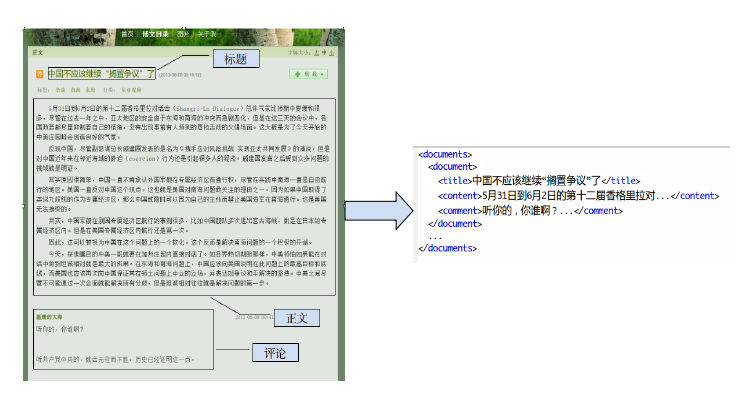
\includegraphics[width=\textwidth]{intro01/blog-to-xml}
  \caption{用XML存储博客的正文,标题和评论}
  \label{intro:fig:blog-to-xml}
\end{figure}

\subsection{HTML文档的模板}
\label{sec:htmltemplateintro}
互联网上有成千上万的HTML文档,对于大部分的网站来说,不可能针对每一个网页单独写一
个静态网页存储到服务器。实际上,我们在互联网上浏览的大部分HTML网页都是通过网站的
后台程序动态生成的,只有极少量的还是通过静态HTML方式进行存储。

在Web开发领域,MVC(Model, View, Controller)模式是目前最流行的开发方法。模型
(Model)是对底层数据和业务的进行的封装;视图(View)负责用户界面的交互,包括给用
户发送信息,接受用户输入等;控制器(Controller)则是系统的控制逻辑,对用户请求进
行处理,用选择合适的视图用于显示模型返回的数据。
如\reffig{intro:fig:mvc}所示\footnote{来
  源:http://en.wikipedia.org/wiki/Model\%E2\%80\%93view\%E2\%80\%93controller}。
目前有很多基于MVC模式的Web开发框架,比如基于Ruby语言的Ruby on Rails,基于Python语
言的Django以及基于Scala语言的Play! Framework等等。这些框架用模型对底层的数据库进
行包装,当用户请求一个HTML页面的时候,控制器负责从数据库中查询相应数据,然后在视
图层选择合适的渲染模板,将对应的数据填充到模板中,从而生成目标HTML文档,将其返回
给用户。\reffig{intro:fig:django}是一个简单的用Django开发网站时视图层的模板示例,
其中\texttt{news.title}和\texttt{news.content}是从数据库中得到的查询结果。
\begin{figure}
  \begin{minipage}[t]{0.5\linewidth}
  \centering
  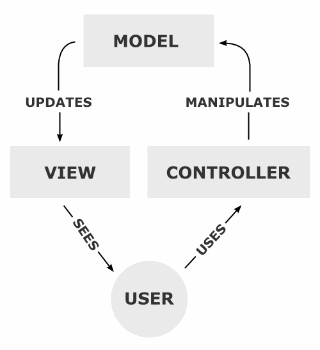
\includegraphics[width=0.5\textwidth]{intro01/MVC-Process}
  \caption{MVC模式}
  \label{intro:fig:mvc}
  \end{minipage}
  \begin{minipage}[t]{0.5\linewidth}
  \centering
  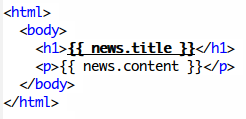
\includegraphics[width=0.6\textwidth]{intro01/django}
  \caption{Django中的HTML模板示例}
  \label{intro:fig:django}
  \end{minipage}
\end{figure}

我们注意到,大部分HTML网页都是通过这种查询底层数据库得到相应数据,然后使用模板进
行渲染的方法生成的。对于大量的从同一个模板生成的网页来说,“模板”就是这些网页
的“公共部分”。实际上,模板的定义要比这里所说的网页的“公共部分”要复杂一些,许
多Web开发框架的模板引擎都支持一些简单的控制结构(如if,for等),如果生成模板的时
候使用了这些控制逻辑,对应的模板也会比较复杂,如\reffig{intro:fig:django-hard}所
示。我们在~\ref{chap:template}中将会给出一个较为严格的定义,这里我们先使用这种直
观的定义便于理解。如果我们能够从大量的由同一个模板生成的网页中将它们的模板抽取出
来,那么我们就可以用抽取出来的模板对其他的由同一个模板生成的网页进行内容的抽取。
简单来说,有了网页的模板以后,每个网页中非“模板”的部分即可以认为是通过查询后台
数据库得到的数据动态生成的,而这些数据正是我们所需要提取出来的。
\begin{figure}
  \centering
  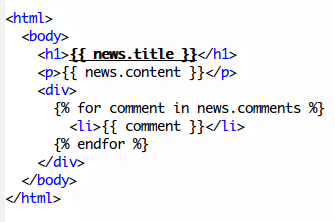
\includegraphics[width=0.5\textwidth]{intro01/django-hard}
  \caption{使用了for的Django模板示例}
  \label{intro:fig:django-hard}
\end{figure}
\section{主要内容与相关工作}
\subsection{主要内容}
\label{sec:mainwork}
本文的主要工作是从已经抓取的大量的网页数据中,自动地对其中的网页进行聚类,得到不
同的类别。对于其中的每一类,将其中可能的模板抽取出来,然后再利用这些模板去抽取新
抓取的网页。由于我们的数据量比较大,因此需要设计一些高效的算法进行抽取;同时,海
量数据也提供了较多的冗余性,使得其中一些隐藏的模式和信息可以更好地被挖掘出来,得
到比较好的实验结果。

互联网上有大量的网站,每个网站的网页都可能采用不同的模板生成。实际上,即使对于同
一个网站,也可能有多个不同的模板。因此,先对这些数据进行聚类是非常必要的,可以尽
早分开相互之间有很大差异的模板所生成的网页。参考~\ref{sec:htmltemplateintro}所述
的网站后台利用模板生成网页过程,我们认为由相同的模板生成的网页,其相似程度主要体
现在仅由HTML标签本身所组成的网页的结构上。我们称这个相似度为网页的结构相似度。与
之类似,HTML文档中所包含的除标签本身以外的内容信息的相似度我们称之为内容相似度。
由于HTML文档中的内容主要来源于后台数据库中查询得到的结果,而数据库中存储的数据本
身没有很大的联系,因此同一模板生成的网页不一定有很高的内容相似度。考虑到这一点,
我们将主要考察HTML文档之间的结构相似度。

在模板提取方面,参考网页后台模板的生成,我们决定主要考虑网页结构上的模板,即由
HTML的标签组成的模板,不考虑HTML文档所包含的内容的相似度。
\subsection{相关工作}
\label{sec:relatedwork}
我们采用基于网页结构相似度的方法进行聚类,
\section{本章总结}
\label{sec:summaryintro}


%%% Local Variables: 
%%% mode: latex
%%% TeX-master: "../main"
%%% End: 



\chapter{系统框架}
\label{chap:framework}
\section{整体框架介绍}
\label{sec:wholeframework}
本文的主要工作在于搭建一个自动的网页模板抽取系统。系统主要分为三个模块:“预处理
模块”,“网页聚类模块”和“网页模板生成和内容提取模块”。从输入的网页集合开始,
依次经过以上三个模块,生成模板后用于提取新的网页中的信息,然后将提取的信息以XML的
格式输出成格式化数据。

整体的框架示意如\reffig{framework:fig:framework}所
示,\reffig{framework:fig:framework}包括了系统的训练和测试。其中,系统训练的输入
是目前已经从互联网上所获得的网页集合,训练的输出为这些网页集合所对应的模板,这部
分系统是离线的。系统的测试输入为新的网页,测试的输出为XML格式的数据,这部分是在线
的。

\begin{figure}
  \centering
  \begin{tikzpicture}[scale=.58,transform shape,
    font=\large,
    io/.style={fill=black!30, text width=3cm, minimum size=1cm,align=center,draw=black},
    submodule/.style={fill=cyan!80, text width=3cm, minimum size=1cm, rounded corners,align=center,draw=black},
    bold arrow/.style={very thick, >=triangle 90},
    input arrow/.style={single arrow, minimum width=5mm, minimum height=0.8cm, draw},
    mylabel/.style={dotted, draw}
    ]    
    \node (input) [io] {输入网页};
    \node (input-arrow) [below=1mm of input, input arrow, shape border rotate=270]{};
    \node (m1-1) [submodule, below=4mm of input-arrow]{过滤无用网页};
    \node (m1-2) [submodule, below=5mm of m1-1]{简化HTML文档} edge[<-] (m1-1);
    \node (m2-1) [submodule, below=1.2cm of m1-2]{结构相似度计算};
    \draw [<-, bold arrow] (m2-1) -- (m1-2);
    \node (m2-2) [submodule, below=5mm of m2-1]{网页聚类} edge[<-] (m2-1);
    \node (m3-1) [submodule, below=1.2cm of m2-2]{模板生成};
    \draw [<-, bold arrow] (m3-1) -- (m2-2);
    \node (m3-2) [submodule, below=5mm of m3-1]{内容抽取} edge[<-] (m3-1);
    \node (new-input-arrow)[left=5mm of m3-2, input arrow]{};
    \node (new-input) [io, left=2mm of new-input-arrow]{新的网页输入};
    \node (output) [io, below=of m3-2]{XML输出};
    \draw [<-, bold arrow] (output) -- (m3-2);
  \begin{pgfonlayer}{background}
    \tikzset{module/.style={inner sep=1em, fill=white, fill=green!30, rounded corners}};
    \node (m1)[module, fit=(m1-1) (m1-2)]{};
    \node (m1-name) [right=5mm of m1]{\Large{预处理模块}};
    \node (m2)[module, fit=(m2-1) (m2-2)]{} [below=of m1];
    \node (m2-name) [right=5mm of m2]{\Large{网页聚类模块}};
    \node (m3)[module, fit=(m3-1) (m3-2)]{} [below=of m2];
    \node (m3-name) [right=5mm of m3] {\Large{模板生成和内容提取模块}};
  \end{pgfonlayer}  
\end{tikzpicture}
  \caption{系统整体框架示意}
  \label{framework:fig:framework}
\end{figure}

以下将逐个介绍各个模块的总体设计。
\section{预处理模块}
\label{sec:filterintro}
预处理模块主要以下分为两个子模块:过滤无用网页和简化HTML文档。
\subsection{过滤无用网页}
\label{sec:filterintro-useless}
我们获得的网页数据主要分为以下几种:目录页、详细页、404及其他错误页。在我们的实验
中,我们只关心详细页的集合,因此,需要首先过滤掉目录页和错误页等无用的网页。

这部分要求要有较快的运行速度,因此不需要设计非常复杂的算法,主要通过设置一些简单
的规则去对原始的网页集合进行过滤。通过观察,我们主要采取了以下这些策略:
\begin{itemize}
\item 404及其他类似的错误页可以通过一些关键字如{404 Not
    Found}或者{Server Error}等进行辨别。通常这些错误页的文档都很简单,长度
  很短,因此还可以通过设置长度阈值将其过滤;这样还可以将一些无用的太短的文档同时
  去除。
\item 大部分目录页的URL和详细页的URL有明显区别。比如对于新浪博客来说,详细页的
  URL都以{.html}结尾,而目录页则没有。例如以下两个URL:
http://blog.sina.com.cn/u/1439351555\\
http://blog.sina.com.cn/s/blog\_55cac30301016yb1.html\\
第一个URL对应的是某个博主的文章目录,第二个URL则是该博主的某篇文章。因此只需要通
过正则表达式匹配的方式即可将目录页过滤。其他网站也有类似这样的规则,我们只需要在
实验前针对每个网站提前设置好规则进行过滤即可。由于每个网站每种特定的网页只需要指
定一种规则,人工的工作量并不大。
\item 为了实验的完备性和对一些特殊的网站进行处理,比如可能存在某些网站,目录页
  的URL和详细页的URL在模式没有太大的区别,或者人工设置规则的办法太麻烦了,我们的
  系统中也实现了通过网页的特征过滤详细页的机制。注意到目录页的作用主要是给用户提
  供进入各个详细页的入口,因此目录页的HTML文档的主要部分是由列表环
  境{<ul>}或{<ol>}中的列表项{<li>}及其包含的超链接标
  签{<a>}组成。\reffig{framework:fig:baidunews}是简化后的百度新闻目录
  页HTML代码的一部分\footnote{来源:2013年6月9日15时的news.baidu.com页面}。我们提
  取出网页中的所有{<li>}标签中的{<a>}标签,计算这些{<a>}标签
  的文本内容占网页所有文本内容的比重,超过一定的阈值则判定为目录页。由于这种方法
  比上述使用简单规则的办法要慢许多,因此在系统中我们将优先使用规则的方法对目录页
  进行过滤。
\end{itemize}
\begin{figure}
  \centering
  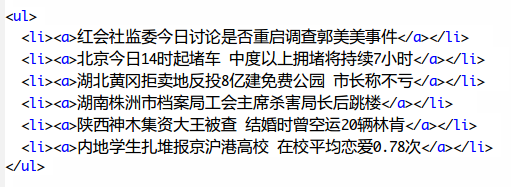
\includegraphics[width=0.5\textwidth]{framework02/baidunews}
  \caption{简化的百度新闻目录页的一部分HTML代码}
  \label{framework:fig:baidunews}
\end{figure}

通过这些策略将目录页和错误页过滤完以后,我们可以得到网页的详细页集合,将其作为下
一个子模块的输入。
\subsection{简化HTML文档}
我们将分多个步骤对HTML文档进行简化。

第一步是去除无用的标签。这些标签有以下特点:
\begin{enumerate}
 \item\label{item:1} 与网页模块无关。去除这些标签时,可以将标签本身及标签的内容一同去掉。比如
  {<script>}、{<link>}、{<style>}等。
\item\label{item:2} 通常是深层次的HTML文档的节点,用于控制格式,在模板中意义不大。
  去除这些标签时只取出标签本身,保留标签所包含的内容。比
  如{<br/>}、{<p>}、{<strong>}、{<em>}等。
\item\label{item:3} 我们在实验中不考虑非文本标签,因此将{<img>}、
  {<audio>}等直接去除。
\item\label{item:4} 最后是去除一些在模板中变化很大的太复杂的标签,典型的是表格相
  关的一些标签,包
  括{<table>}、{<th>}、{<tr>}、{<td>}等。
\end{enumerate}

接下来我们把每个HTML文档都解析成DOM Tree。DOM Tree的构建速度比较慢,在解析时需要
将整个HTML同时载入内存,占用较多的内存资源,可能导致我们在需要处理的数据量较大时
会出现一定的问题。去除这些无用标签可以加快HTML解析成DOM Tree的速度,减小内存占用,
也减小了后续的模板聚类和模板检测中的噪音,是很有必要的。

第二步是对解析好的DOM Tree进行简化。由于在树形结构上做相关的操作较为复杂,我们首
先将树形结构转化为更便于处理的序列形式。具体地,我们采用先序遍历的方式,将DOM
Tree转化成一个标签序列,为了可以还原成原始的DOM Tree,我们在遍历的同时在每个节点
处保存了该节点的深度信息。对于\reffig{framework:fig:html}所示的HTML文档,解析成
的DOM Tree如\reffig{framework:fig:domtree}所示,如果每个标签采用{标签名+深
  度}的表示方法,则我们采用先序遍历方式可以得到该DOM Tree对应的序列
为:{<html0><body1><div2><a3><p3><div2>}。先序遍历的优点在于可以保证每个子
树的所有节点在序列中的位置是连续的,且根节点位于这段连续子序列的起始处。比如以第
一个{<div>}标签为根的子树在遍历得到的序列中对应的序列
为{<div2><a3><p3>},根节点{<div2>}位于子序列的起始位置。这些特点对
于后续的处理有很大的帮助。

第三步是对HTML文档中重复出现的记录进行检测,去掉重复的多余的部分,从而用更简单的
方式表示原文档。我们将DOM Tree的某个子树成为一个“记录”。由于HTML模板中动态生成
的部分中可能包含大量重复的模式,比如\reffig{intro:fig:django-hard}所示的Django模
板,其中的{news.comments}可能包含不定数目的元素,在比较由这个模板生成的两
个不同网页的时候,应该将其中数目可能不一样的{<li>}的结构视为一样,否则将对
后续的处理造成较大的误差。在网页的生成中,这种重复模式是大量存在的,因此,检测网
页中的重复记录并做相应的简化是预处理过程中最重要的一个部分,我们将在
第~\ref{chap:suffixtree}章中详细介绍。
\begin{figure}
  \begin{minipage}[t]{0.5\linewidth}
  \centering
  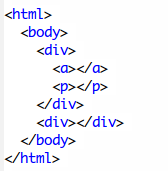
\includegraphics[width=0.5\textwidth]{framework02/framework-html}
  \caption{一个简单的HTML文件}
  \label{framework:fig:html}
\end{minipage}
\begin{minipage}[t]{0.5\linewidth}
  \centering
  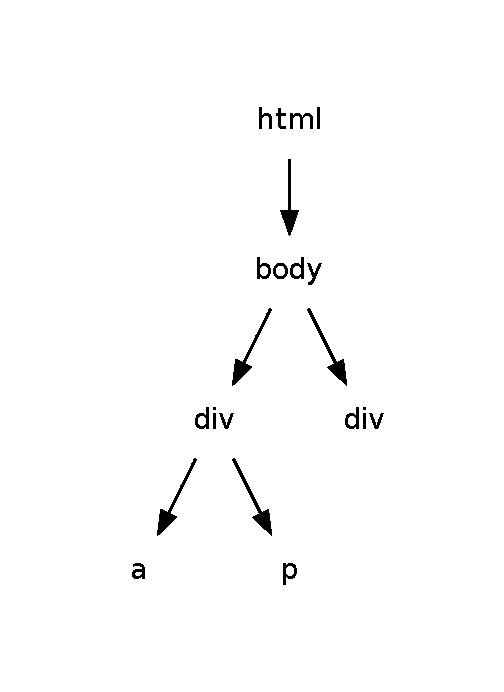
\includegraphics[width=0.5\textwidth]{framework02/domtree}
  \caption{\reffig{framework:fig:html}对应的DOM Tree}
  \label{framework:fig:domtree}
\end{minipage}
\end{figure}
\section{网页聚类模块}
\label{sec:clusterintro}
这个模块包含两个主要的子模块:计算网页结构相似度和实现网页聚类算法。

通过网页的预处理模块,我们将得到一个简化的由DOM Tree先序遍历得到的序列,其中不包
含重复的记录。为了能够进行聚类,我们首先需要计算每个文档之间的结构相似度。这里我
们采用的是基于最长公共子序列(Longest Common Sequence)的方法,简称LCS。实际上,我们
整个工作中与序列处理相关的工作很多都将基于LCS,包括后面的模板生成和内容提取模块。
我们将对每两个文档都计算一次LCS,得到文档之间的结构相似度,将其用于后续的聚类。

在聚类子模块,有几个特点值得我们注意:
\begin{itemize}
\item 网页中的模板个数即最终聚类的个数事先是不知道的,因此我们不能采用一些类似
  于K-means等需要预先设定聚类的个数的算法。
\item 网页数量很大,需要有较快的执行速度。
\item 我们可以利用的信息只有网页文档两两之间的结构相似度。
\end{itemize}

我们将采用简单的层次聚类的方法,通过设置阈值的方法控制聚类的类别个数。这个模块的
具体实现将在第~\ref{chap:cluster}章中详细介绍。
\section{模板生成和内容提取模块}
\label{sec:templateintro}
这个模块是本次实验中最主要的部分,包括两个子模块:模板生成和内容提取。

在模板生成子模块中,我们将从之前聚好的类中提取出每个类对应的模板。模板的提取将仍
然基于DOM Tree先序遍历得到的序列和LCS,并利用无监督的方法来进行构建。这个子模块输
出的模板将作为整个系统的训练模块的输出。

为了能够从网页中提取出我们所需要的部分,我们还需要人工对模板中的某些部分指定语义,
比如对于新闻来说,模板中的哪些部分将对应新闻标题、正文、评论等。由于模板的数量不
会很多,这部分的工作量不会很大。

内容提取子模块将利用之前训练得到的聚类信息和模板,选择合适的模板从新的网页中提取
出我们需要的信息,并将这个信息以XML格式输出成结构化的数据。

这个模块我们将在第~\ref{chap:template}章中进行详细介绍。
\section{本章小结}
\label{sec:summaryframework}
本章首先简单介绍了系统的整体框架,然后分别对每个模块的总体设计进行了说明。其中我
们重点介绍了预处理模块中除了重复记录检测子模块以外的部分,其他概述的部分,如重复
记录的检测,网页的聚类,模板生成和内容提取等,我们将在后续章节中一一详细介绍。

%%% Local Variables: 
%%% mode: latex
%%% TeX-master: "../main"
%%% End: 


\chapter{基于后缀树的重复记录检测}
\label{chap:suffixtree}

\section{后缀树简介}
\label{sec:suffixtreeintro}
后缀树(Suffix Tree)是一种可以快速高效实现许多字符串操作的数据结构。Weiner最早
在\cite{weiner1973linear}中提出了后缀树的概念,Ukkonen在\cite{ukkonen1995line}中
提出了一个$O(n)$时间复杂度的在线构造算法。

后缀树实际上是前缀树(Trie树)的一种特殊形式。后缀树的每一条边都代表着一个序列,从
根节点到后缀树叶子节点的每条路径都对应着原序列的一个后缀。也就是说,后缀树其实就
是由序列所有后缀所组成的前缀树。举个例子,对于字符串\texttt{APPLE},其所有的后缀
为:
\begin{verbatim}
APPLE
PPLE
PLE
LE
E
\end{verbatim}
对应的后缀树如\reffig{suffixtree:fig:suffix-tree-apple}所示。
从\reffig{suffixtree:fig:suffix-tree-apple}中可以看到,共有5条从根节点到叶子节点
的路径,每一条路径都对应于一条后缀。
\begin{figure}
  \centering
  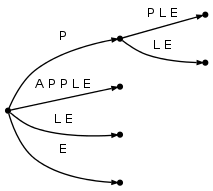
\includegraphics[width=0.5\textwidth]{suffixtree03/suffix-tree-apple}
  \caption{APPLE对应的后缀树}
  \label{suffixtree:fig:suffix-tree-apple}
\end{figure}

我们可以总结出序列$S$的后缀树有以下几个特点:
\begin{enumerate}
\item 所有的边都对应\texttt{S}的长度至少为一的非空的子序列
\item 从根到叶子节点的路径序列和序列S的后缀一一对应
\item 所有的内部节点(根节点不一定)都有至少两个子节点
\end{enumerate}

\section{Ukkonen后缀树构建算法}
\label{sec:ukkonen}
最简单的后缀树算法是先取出序列所有的后缀,然后按照前缀树的构造方法构造序列的后缀
树。这种方法虽然简单,但是复杂度较高,不适用于数据量较大的情况。为了高效地实现重
复记录检测的模块,我们的系统实现了Ukkonen在\cite{ukkonen1995line}中提出的时间复杂
度为$O(n)$的后缀树在线构建算法。以下将以字符串\texttt{BANANA}为例,简单介绍这种在
线算法的构造过程。由于这个算法比较复杂,以下的这个例子并不能涵盖算法的所有细节。

首先我们引入3个状态变量描述某一个时刻对应的后缀树的构造状态。

第一个状态变量是\texttt{\#},表示序列中即将扫描的下一个元素的位置。初始值为0,表
示第一个元素,在以后的每轮迭代中,\#的值将加1,当\#的值和序列的长度相同时迭代终
止。
  
第二个是\texttt{activePoint},用于表示下一次要在后缀树插入新的点时的位置,为了确
定这样一个唯一的位置,我们需要一个三元组\texttt{(activeNode, activeEdge,
  activeLength)}表示\texttt{activePoint},这三个变量分别表示当前后缀树的某个节点,
该节点的某条边以及这条边上第几个元素。初始值为\texttt{(root, '', 0)},表示初始的
插入操作都在根节点\texttt{root}上进行。下面
以\reffig{suffixtree:fig:suffix-tree-apple}中的后缀树为例简要说明:若
用\texttt{root}表示根节点,则当\texttt{activePoint}为\texttt{(root, A, 3)}时意味
着下一次插入新的点的位置应该是从根节点\texttt{root}的以字母\texttt{A}开头的边的
第3个字符后面,即\texttt{root}的\texttt{APPLE}对应的边的第二个\texttt{P}字母后面
的位置。
  
第三个状态变量是\texttt{remainder},表示当前还需要往后缀树中插入几次后缀。初始值
为1。

对于我们的输入\texttt{BANANA}来说,最后一个字母是\texttt{A},这个字母在字符串之前
的某个位置中出现过(\texttt{BANANA}共有3个字母\texttt{A}),因此需要在输入串的末
尾增加一个终结符,以保证输入的最后一个字符没有在之前出现过,我们这里采用\$。因此,
原始的输入\texttt{BANANA}就变成了\texttt{BANANA\$}

一开始的时候,我们只有一个根节点,\#为0,插入后缀\texttt{B},变
成\reffig{suffixtree:fig:1}所示的图;下一轮迭代\#值增加到1,新的后缀\texttt{A}在
原来的边中没有出现,插入一条新的边,得到\reffig{suffixtree:fig:2};接下来\#增加
到2,和前一步一样,新的后缀\texttt{N}没有在原来的边中出现过,插入一条新的边,得
到\reffig{suffixtree:fig:3}。目前为止,\texttt{activePoint}和\texttt{remainder}都
没发生变化。

接下来\#加1,将导致需要插入一条新的后缀\texttt{A},但是我们发现\texttt{A}已经在之
前的边中出现过,因此这时我们不插入新的边,而将\texttt{activePoint}更新
为\texttt{(root,A,1)},\texttt{remainder}加1,此时后缀树
如\reffig{suffixtree:fig:4}所示,边数没有发生变化,但是状态变量发生了改变。下一
步\#再加1,由于此时\texttt{remainder}为2,因此我们需要将新的后缀\texttt{N}往后缀
树中插入两次。从\texttt{activePoint}出发,我们发现下一个字母正好是\texttt{N},因
此我们不再试图往后缀树中插入\texttt{N}了,而是
将\texttt{activePoint}和\texttt{remainder}分别更新为\texttt{(root,A,2)}和3。下一
轮迭代也是类似,在插入最后一个\$之前,后缀树如\reffig{suffixtree:fig:6}所示,
\texttt{activePoint}和\texttt{remainder}的值分别为\texttt{(root, A, 3)}和4。
% 插入后缀树构造的图片

\begin{figure}
  \begin{subfigure}[t]{0.33\linewidth}
    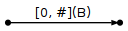
\includegraphics[width=0.8\textwidth]{suffixtree03/suffixtree-1}
    \caption{\#=0}
    \label{suffixtree:fig:1}
  \end{subfigure}
  \begin{subfigure}[t]{0.33\linewidth}
    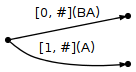
\includegraphics[width=0.8\textwidth]{suffixtree03/suffixtree-2}
        \caption{\#=1}
    \label{suffixtree:fig:2}
  \end{subfigure}
    \begin{subfigure}[t]{0.33\linewidth}
    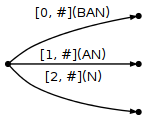
\includegraphics[width=0.8\textwidth]{suffixtree03/suffixtree-3}
        \caption{\#=2}
    \label{suffixtree:fig:3}
  \end{subfigure}
  \begin{subfigure}[t]{0.33\linewidth}
    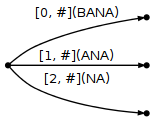
\includegraphics[width=0.8\textwidth]{suffixtree03/suffixtree-4}
    \caption{\#=3}
    \label{suffixtree:fig:4}
  \end{subfigure}
  \begin{subfigure}[t]{0.33\linewidth}
    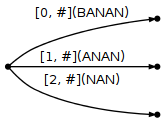
\includegraphics[width=0.8\textwidth]{suffixtree03/suffixtree-5}
        \caption{\#=4}
    \label{suffixtree:fig:5}
  \end{subfigure}
    \begin{subfigure}[t]{0.33\linewidth}
    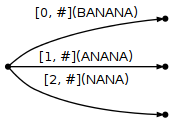
\includegraphics[width=0.8\textwidth]{suffixtree03/suffixtree-6}
        \caption{\#=5}
    \label{suffixtree:fig:6}
  \end{subfigure}
  \caption{前六轮迭代(\#从0到5)中的后缀树变化}
  \label{suffixtree:fig:0to5}
\end{figure}
\begin{figure}
  \begin{subfigure}[t]{0.5\linewidth}
    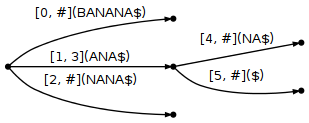
\includegraphics[width=\textwidth]{suffixtree03/suffixtree-7-1}
    \caption{remainder=4}
    \label{suffixtree:fig:7-1}
  \end{subfigure}
  \begin{subfigure}[t]{0.5\linewidth}
    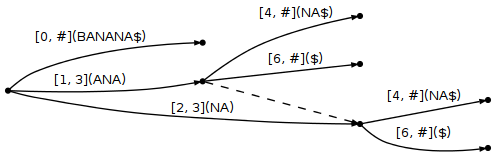
\includegraphics[width=\textwidth]{suffixtree03/suffixtree-7-2}
        \caption{remainder=3}
    \label{suffixtree:fig:7-2}
  \end{subfigure}
  \begin{subfigure}[t]{0.5\textwidth}
    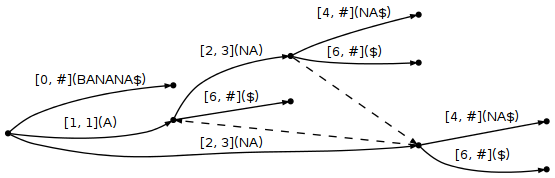
\includegraphics[width=\textwidth]{suffixtree03/suffixtree-7-3}
    \caption{remainder=2}
    \label{suffixtree:fig:7-3}
  \end{subfigure}
  \begin{subfigure}[t]{0.5\textwidth}
    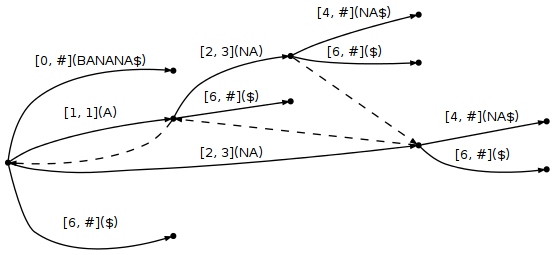
\includegraphics[width=\textwidth]{suffixtree03/suffixtree-7-4}
    \caption{remainder=1}
    \label{suffixtree:fig:7-4}
\end{subfigure}
\caption{最后一轮迭代(\#=6)时的后缀树}
\label{suffixtree:fig:7}
\end{figure}

%%% Local Variables: 
%%% mode: latex
%%% TeX-master: "../main"
%%% End: 


最后一轮迭代,我们需要插入终止符\$。从此时的\texttt{activePoint}出发,发现下一个
字母和和\$并不匹配,此时我们需要往后缀树中插入\$字符,方法是
在\texttt{activePoint}对应的位置生成一个新的内部节点,并在新生成的节点的地方插入
一条边,表示\$,如\reffig{suffixtree:fig:7}所示。我们需要更
新\texttt{activePoint}的值:将\texttt{activeNode}移到根节点处(在这个例子中实际上
没有移动),对应的边是以原来的\texttt{activeEdge}的第2个字母开头的边,
即\texttt{N},\texttt{activeLength}减1。\texttt{remainder}的值也减1,变为3,也就
是我们还需要插入3次\$。接下来的两次插入和我们第一次插入时的情况一样,会新生成两个
内部节点;最后一次插入则和一开始的情况一样,我们直接在根节点处插入\$。最后一轮迭
代的过程如\reffig{suffixtree:fig:7}所示,最后生成的完整的后缀树
如\reffig{suffixtree:fig:7-4}所示。

在最后的\reffig{suffixtree:fig:7-4}中,我们看到还有一些连接几个内部节点之间的有向
的虚线,我们之前没有提到,这是后缀链(Suffix Link)。我们例子中的后缀链都是在最后
一轮迭代插入\$时生成的。关于后缀链生成的简单的规则是:在同一轮迭代中,如果在某一
步中某个节点处发生了一次插入,则要从这一轮迭代之前生成内部节点(如果有的话)引一
条后缀链指向该节点。后缀链的作用是如果在某个带有后缀链的节点发生了插入,则在更
新\texttt{activePoint}时把其中的\texttt{activeNode}更新为沿着后缀链连接的那个节点,
而不是根节点。后缀链不影响前述的其他规则。限于篇幅,我们不再具体举例说明后缀链的
使用方法。

\section{重复记录检测算法}
\label{sec:multipldetect}

\subsection{后缀树检测重复序列的基本算法}
依照~\ref{sec:ukkonen}所述的后缀树构造算法,我们给每一个DOM Tree的先序遍历序列构
造一个后缀树,然后根据后缀树检测其中重复的记录。

根据后缀树构造的特点,任意一条从根节点到内部节点的路径组成的序列都是原序列中重复
出现的子序列,且重复的次数是以该内部节点为根的子树的叶子节点个数。
在\reffig{suffixtree:fig:7-4}中,\texttt{A},\texttt{ANA},\texttt{NA}都是
\texttt{BANANA}的重复子串,分别重复出现了3次,2次和2次。这种方法有以下几个问题:
\begin{itemize}
\item 不同的重复子串之间可能有包含或者相交的关系。在之前的例子中,\texttt{ANA}包
  含了\texttt{NA}和\texttt{A}。
\item 同一个重复子串在原序列上有交集。比如\texttt{ANA},对应到原序列上的两个子序
  列有交集\texttt{A}。  
\end{itemize}

直接采用上面的方法查找后缀树中的重复记录是不可行的。我们从DOM Tree得到先序遍历序
列和普通的序列不一样,里面是包含有原始的树的结构信息的。我们需要检测的重复记录必
须位于同一个子树上,有公共的父亲。这个特点对应到序列上,必须要求:
\begin{itemize}
\item 重复序列不能横跨两个子树
\item 重复序列必须有公共的父亲
\end{itemize}

此外,我们还要求这个重复序列必须尽可能地长。

\subsection{改进的检测算法}
因此,我们需要进一步对原来的重复序列查找算法进行改进。算
法~\ref{suffixtree:algo:fromroot}和\ref{suffixtree:algo:findrep}给出了我们查找所
有符合我们要求的重复子序列的算法。

% 输入代码文件
\begin{algorithm}
  \caption{从根节点出发,找出所有的重复子序列\label{suffixtree:algo:fromroot}}
  \begin{algorithmic}[1]
    \Require 已经构建好的后缀树,根为$root$
    \Ensure 该后缀树中所有的重复子序列
    \State $//$从节点出发,寻找所有的重复子序列
    \For{$edge \gets root.edges~\mathbf{if}~edge.endNode.isNotLeaf$}
    \State $//$取后缀树根节点的每条边的第一个元素作为每个子树的根节点
    \State $subTreeRoot := edge.firstElement$
    \State $//$查找以该节点为根的所有重复子序列
    \State findAllRepetitions$(root, \mathbf{nil}, subTreeRoot)$
    \EndFor
  \end{algorithmic}
\end{algorithm}

\begin{algorithm}
  \caption{找出后缀树中经过某个内部节点的所有可能的重复子序列}
  \label{suffixtree:algo:findrep}
  \begin{algorithmic}[1]
    \Require 一个内部节点$node$,当前已经找到的重复序列$prefix$,要找的
    子树的根节点$subTreeRoot$
    \Ensure 所有经过该内部节点的符合要求的重复序列
    \Function {findAllRepetitions}{$node, prefix, subTreeRoot$}
    \State $//$定义一个空集合
    \State $results := Collection.empty$
    \State $//$对于该内部节点的每一条不连接叶子节点的边
    \For{$edge \gets node.edges~\mathbf{if}~edge.endNode.isNotLeaf$}
    \State $//$依次取出该条边上元素的根节点可能为root的点
    \State $seq := edge.takeWhile(element$ inSubTreeOf $subTreeRoot)$\label{suffixtree:code:equals}
    \If {$seq.length == edge.length$}
    \State $//$遍历完了该条边上所有元素,
    \State $//$则取该条边连接的下一个内部节点进行递归查找
    \State findAllRepetitions($edge.endNode, prefix + seq, subTreeRoot$)
    \Else
    \State $//$否则,将当前得到的序列加入到结果集合中
    \State addToResults$(prefix + seq, results)$\label{suffixtree:code:add}
    \EndIf
    \EndFor
    \State \Return{$results$}
    \EndFunction
    \State
  \end{algorithmic}
\end{algorithm}

%%% Local Variables: 
%%% mode: latex
%%% TeX-master: "../main"
%%% End: 


根据算法~\ref{suffixtree:algo:fromroot}和~\ref{suffixtree:algo:findrep}得到的重复
子序列,可以保证不会横跨两个子树,且尽可能地长,但还有几点需要说明。

第一,根据算法~\ref{suffixtree:algo:fromroot}和~\ref{suffixtree:algo:findrep}得到
的在原序列中重复出现的子树的序列,不一定有相同的父亲节点,因此不能直接根据这个结
果去掉重复记录,还需要做进一步的处理。

第二,算法~\ref{suffixtree:algo:findrep}中的代码addToResults$(prefix + seq,
results)$将新的序列加入到结果集合中。实际在加入的时候,我们需要先将新的序列和结果
集合中已有的序列进行对比。如果结果集合中的某个序列被新的序列所包含,则我们用新的
序列代替原有的序列。这个操作可以在$O(1)$的时间内完成。因为在后缀树中,如果两个子
序列有包含关系,即$S_1$包含$S_2$,必然有$S_2$为$S_1$的后缀,这可以通过比
较$S_1$和$S_2$最后一个元素的下标是否相等来判断。

\subsection{合并重复记录}
接下来我们将对找出来的所有可能的重复序列进行合并。根据先序遍历的特点,子树的根节
点总是出现在该子树对应的序列的起始处。因此,对于我们找到的每一个重复的子序列,我
们总是可以通过向前搜索找到其父节点。接下来把所有的序列按照其父亲节点进行分类,然
后遍历每一个父节点所对应的全部重复序列$S_1,S_2,...,S_n$,若存在一个序列集
合${S_{i_1},S_{i_2},...,S_{i_k}}, i_1<i_2<...<i_k, k>1$,其中的每个序列都相等,则
只保留$S_{i_1}$,将其余全部去除。最后我们将在保留下来的$S_{i_1}$中设定标志位,表
明该序列在模板中是可以多次出现的。

我们实际的合并算法要比上述的稍复杂一些,因为有很多边界情况需要特殊处理。比如,算
法~\ref{suffixtree:algo:fromroot}和\ref{suffixtree:algo:findrep}虽然去除了序列横
跨两个子树和序列互相包含的问题,但是对于序列相交的情况,并没有做相应的处理。对于
以下的某个HTML标签序列片段(每个标签由\texttt{标签名+深度}组成):
\begin{verbatim}
...<div3><div4><div3><div4><a5><img5><div4><a5><img5>...
\end{verbatim}
按照之前的算法,我们可以找到的符合条件的重复序列包
括\texttt{<div3><div4>}和\texttt{<div4><a5><img5>}。但是这两个序列实际上有交
集:\texttt{<div4>}。我们采取的策略是只取更深的重复序列。在这个例子中,我们保
留\texttt{<div4><a5><img5>},将第二个\texttt{<div3><div4>}序列从重复序列集合中去
掉。

其他还有一些边界条件,这里不再赘述了。

\section{本章小结}
\label{sec:summarysuffixtree}
本章主要对预处理模块中的重复记录检测子模块进行了详细描述。先简单介绍了后缀树的定
义和性质,然后举了一个具体的例子说明如何在$O(n)$时间内在线构建出一个序列的后缀树,
最后对利用后缀树进行重复记录检测的算法做了详细的介绍和说明。

这个子模块是预处理模块中最重要的一个。如果我们不对网页中重复的记录进行处理,这些
不定个数的重复记录将成为后续的聚类和模板提取过程中很大的噪音,大大减小聚类和模板
提取的精度。由于我们实现并使用了后缀树这种高效的数据结构,使得我们的算法可以很快
找出所有符合条件的重复序列,并将它们正确地进行合并。

%%% Local Variables: 
%%% mode: latex
%%% TeX-master: "../main"
%%% End: 


\chapter{网页相似度计算与聚类}
\label{chap:cluster}

\section{基于最长公共子串的网页距离计算}
\label{sec:lcs}

\section{算法优化与改进}
\label{sec:optimize}

\section{聚类算法实现}
\label{sec:clusteralgo}

\section{本章总结}
\label{sec:summarycluster}


%%% Local Variables: 
%%% mode: latex
%%% TeX-master: "../main"
%%% End: 


\chapter{模板生成和内容提取}
\label{chap:template}
\section{模板定义}
我们在第~\ref{sec:htmltemplateintro}节中介绍了模板直观上的定义:不同网页公共的部
分。我们期望从目前得到的大量的由同一模板生成的网页集合中,找出那些反复出现的网页
结构,将其作为这些网页的模板。

这里我们将首先形式化定义模板的组成。模板的基本元素是基本节点(Base Node),每
个节点有两种形式:
\begin{enumerate}
\item 单个不重复的HTML标签,即$<tag>$
\item 由一个或多个HTML标签组成的序列,这些序列可以出现一次或多
  次,即$(\sum_{i=1}^N<tag_i>)+$,其中$N \ge 1$
\end{enumerate}
这里的$+$表示可以出现一次或者多次,沿用的是正则表达式的习惯。可以看到基本节点与经
过预处理去除重复记录后的序列节点是对应的。第一种基本节点对应没有合并的序列节点,
第二种基本节点对应着多个重复记录合并后的序列节点,由于是一个“记录”,因此可以由
一个或多个标签组成,并且可以重复出现。

基本节点的序列可以组成必选节点(Essential Node)或可选节点(Optional Node)。必选
节点对应着由基本节点组成的一个序列,若基本节点用$tn_i$表示,则必选节点$EN$可以表
示为:
\[
EN=tn_1tn_2...tn_n
\]
可选节点$ON$则同时对应多个序列,每个序列由不同的基本节点组成,同时每个序列还对应
着一个出现概率$p$,即:
\[
ON=(tn_{11}tn_{12}...tn_{1n_1},p_1)|(tn_{21}tn_{22}...tn_{2n_2},p_2)|...|(tn_{k1}tn_{k2}...tn_{kn_k},p_k)
\]
这里$|$表示“或”的关系。

我们规定模板中必选节点和可选节点必须间隔出现,一个模板(Template)$Tp$可以定义为
这样一个序列:
\[
Tp=[ON_0]EN_1ON_1EN_2ON_2......EN_n[ON_n]
\]
其中第一个可选节点$ON_0$和最后一个可选节点$ON_n$都不是必需的。
\section{模板生成}
\label{sec:templategen}
通过聚类,我们已经得到了一些由同一种模板生成的网页集合,接下来我们将对每个聚类单
独进行处理,生成对应的模板。设当前我们处理的聚类为$c$,聚类的中心点
是$p_{center}$,类中的点$p_i$对应的序列为$s_i$。

根据定义,我们需要生成一个必选节点和可选节点交替出现的序列。我们的方法是:先生成
全部的必选节点,然后在中间插入可选节点。

必选节点,顾名思义就是在该模板生成的网页中,必选节点中包含的所有基本节点都应该出
现。因此,我们需要求出在$c$中每个序列都出现的那些标签序列$s_{common}$。做法是从聚
类的中心点$p_{center}$出发,将其对应的序列$s_{center}$作为$s_{common}$的初始值,
依次与$c$中的每一个序列求一次最长公共子序列$lcs$,并将$s_{common}$的值更新
为$lcs$。迭代结束时得到的标签序列就是组成必选节点的所有的基本节点。算法如伪代
码~\ref{template:algo:common}所示。
\begin{algorithm}
  \caption{得到组成必选节点的所有基本节点}
  \label{template:algo:common}
  \begin{algorithmic}[1]
    \Require 输入聚类$c$
    \Ensure 得到$c$中所有文档共有的序列$s_{common}$
    \Function{findCommonSequence}{$c$}
    \State $//$初始化为中心点所对应的序列
    \State $s_{common} := c.s_{center}$
    \State $//$依次求最长公共子序列
    \For{$s_i \gets c.sequences$}
    \State $lcs := getLCS(s_i, s_{common})$
    \State $s_{common} := lcs$
    \EndFor
    \State \Return $s_{common}$
    \EndFunction
  \end{algorithmic}
\end{algorithm}

以上得到的序列只是所有网页结构的公共部分,每个由这个模板生成的网页都应该有这个结
构,然而这并不是模板的全部组成。我们考虑到很多后台模板生成网页时可能会使用一些条
件分支控制结构,如if,因此仅仅由上述的序列组成模板是不够的。仍然以Django为例,有
些网页的标题可能有副标题,而有些可能没有,在Django框架的模板语言中,可以写成
如\reffig{template:fig:django-if}所示的模板片段。根据这个模板的定
义,<h2>标签并不一定会在全部的由该模板生成的网页中出现,但我们在模板生成
的时候必须考虑到这种情况,否则有些内容比如{<h2>}对应的“副标题”就没法正确
提取了。为此,我们引入了可选节点。因为实际的模板中可能会有多种不同的条件分支,所
以每个可选节点对应多个不同的基本节点的序列,这些序列不一定在每个网页中都出现,每
个序列都对应着一定的出现概率。

\begin{figure}
  \centering
  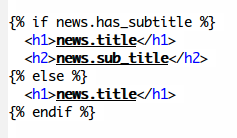
\includegraphics[width=0.3\textwidth]{template05/django-if}
  \caption{Django带条件判断的模板}
  \label{template:fig:django-if}
\end{figure}

以下我们举个简化的例子来说明构造可选节点的基本思想。设有3个序列,分别为:
\begin{eqnarray*}
s_1&=&aorzbcdlxe\\
s_2&=&athubeatcdlxe\\
s_3&=&athubeatcdpkue
\end{eqnarray*}

首先,根据算法~\ref{template:algo:common},得到$s_{common}$为$abcde$。然后,我们
将每个序列同$s_{common}$进行对齐,得到
\[
\begin{matrix}
s_1      &:&\mathbf{a}&orz&\mathbf{b}&   &\mathbf{cd}&lx&\mathbf{e}\\
s_2      &:&\mathbf{a}&thu&\mathbf{b}&eat&\mathbf{cd}&lx&\mathbf{e}\\
s_3      &:&\mathbf{a}&thu&\mathbf{b}&eat&\mathbf{cd}&pku&\mathbf{e}\\
s_{common}&:&\mathbf{a}&   &\mathbf{b}&   &\mathbf{cd}&   &\mathbf{e}
\end{matrix}
\]

我们利用每个序列同$s_{common}$对齐的结果,对每个序列进行分割,我们
用$s_i[t_1,t_2]$表示序列$s_i$在对齐的标签$t_1,t_2$之间的部分,如$s_3[a,b]$表示序
列$thu$。对于每一个区间$[t_1,t_2]$,如果文档集合中的某些序列有未对齐的部分,
即$\exists s_i,|s_i[t_1,t_2]| > 0$,我们将对应生成一个可选节
点$ON_{t_1,t_2}$,这个可选节点对应于这个区间中所有未对齐的子序列。在我们的例
子中,我们生成以下三个可选节点:
\begin{eqnarray*}
  ON_{a,b}&=&thu,2/3~|~orz,1/3\\
  ON_{b,c}&=&eat,2/3\\
  ON_{d,e}&=&lx,2/3~|~pku,1/3
\end{eqnarray*}

对齐的部分则对应生成必选节点,分别为:$a,b,cd,e$。将这些必选节点和可选节点间隔地
依次组成一个序列,这3个序列对应的模板就生成好了。

由以上的例子,我们可以得到模板生成子模块的整体流程图
如\reffig{template:fig:subsystem}所示,
\begin{figure}
  \centering
  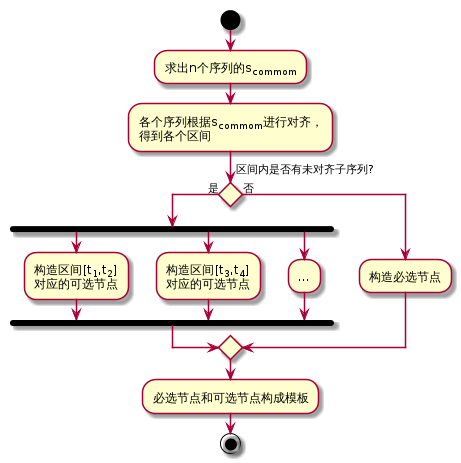
\includegraphics[width=0.7\textwidth]{template05/subsystem}
  \caption{模板生成子模块整体流程图}
  \label{template:fig:subsystem}
\end{figure}

然而,实际的情况却要比上面的例子更复杂一些。对于实际的网页文档集合,区
间$[t_1,t_2]$中未对齐的那些标签子序列,有些可能差异很大,有些则可能非常相近,但不
完全一样。因此,我们需要将\reffig{template:fig:subsystem}中构造可选节点的过程进一
步细化:先将这些子序列中差异较大的几种模式分开,然后针对每个分好的类别提取其中共
有的部分,用于构造可选节点。

根据以上的叙述,我们发现,构造可选节点的这个子问题和我们的系统要解决的问题有很大
的相似性,都可以简单描述为:存在一个序列集合,里面的元素由几种不同的模式生成,需
要先将这些元素分成几种类别,然后针对每个类别去提取公共的部分,即“模板”。对于构
造可选节点这个子问题而言,这里的“模板”指的是在那些子序列的聚类中反复出现的模式,
和我们要最终要提取的网页模板有很大的相似性。为了叙述简便,我们不妨称之为“子模
板”。

提取这些子模板的过程和系统的整体框架极其类似。对于每个存在未对齐子序列的区
间$[t_1,t_2]$:
\begin{enumerate}
\item 区间内所有未对齐的序列组成一个新的序列集合$set_{s'}$。
\item 把集合$set_{s'}$放入之前的聚类模块中,根据算
  法~\ref{cluster:algo:clustering}得到聚类的结果$clusters$。
\item 针对$clusters$中的每个聚类$c$,使用算法~\ref{template:algo:common}得到它
  的“子模板”,并根据聚类$c$的大小和原始文档集合之间的大小,计算这个“子模板”的
  出现概率$p$。
\end{enumerate}

这样,区间$[t_1,t_2]$得到一个由多个子模板和其对应的出现概率组成的序列,这个序列就
组成了区间$[t_1,t_2]$所对应的的可选节点。必选节点则根据对齐结果生成,主要是将一些
连续的中间没有未对齐序列的基本节点合并成一个必选节点,如上面的例子中,我们
将$c,d$两个基本节点合并成了一个必选节点。这些必选节点和可选节点组成的序列也就构成
了我们要处理的这个聚类的模板了。
\begin{figure}
  \centering
  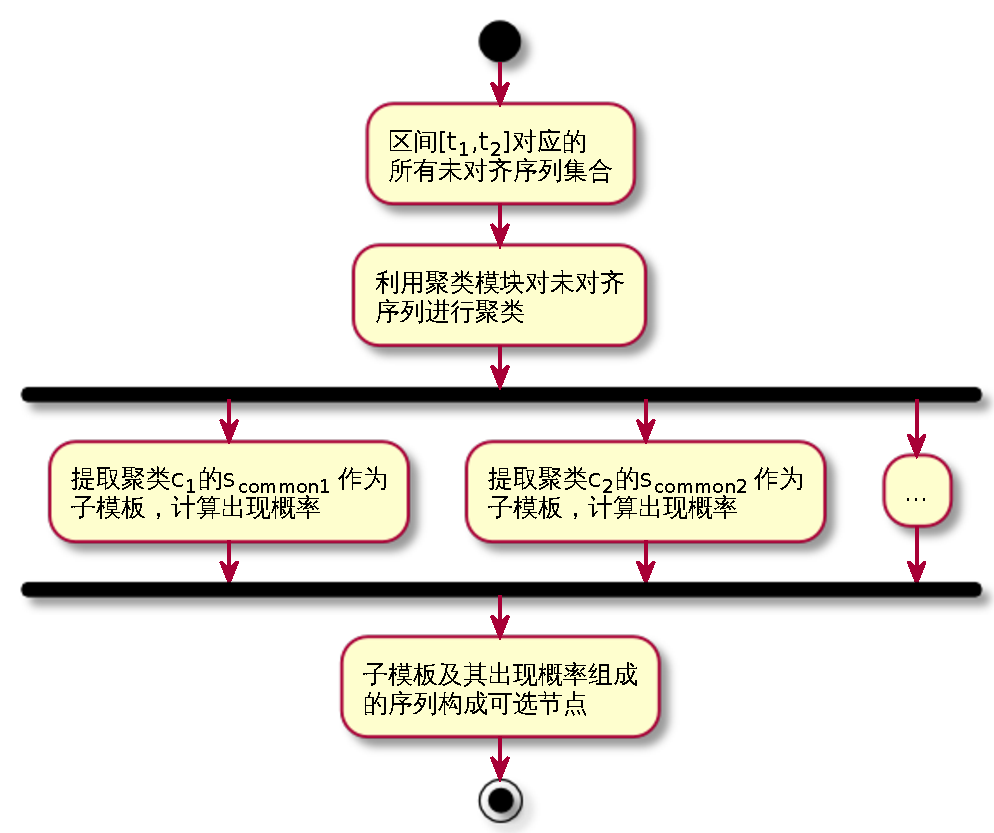
\includegraphics[width=0.7\textwidth]{template05/subtemplate}
  \caption{细化的构造可选节点的流程图}
  \label{template:fig:subtemplate}
\end{figure}

细化以后的构造可选节点的流程如\reffig{template:fig:subtemplate}所示。

最后,观察到从\reffig{template:fig:subsystem}中构造各个可选节点的过程是并行的,因
此为了加快模板的计算速度,我们在这里再次使用了Actor模型并行地计算每个可选节点。

我们对每一个聚类都生成一个模板,这些模板将作为我们系统训练的输出,用于提取新的网
页中的内容。
\section{内容提取}
\label{sec:extraction}
这个子模块中,我们将利用聚类模块得到的聚类和前一个子模块生成好的模板,对新输入的
网页进行内容的提取。

作为内容提取的第一步,我们需要先针对每个模板做一些简单的人工标注。由于整个模板生
成的过程是无监督的,中间也没有考虑模板对应部分的语义信息,因此,在自动生成好模板
后,还需要通过人工指定语义的办法使得系统能够判断哪部分的内容才是我们真正所关心的。
比如当我们生成好了一类新闻网页的模板后,我们可以手工在模板的对应部分标
上“标题”,“正文”和“评论”等,这样后续的内容提取部分就能自动将这些内容提取出
来。

第二步需要先将新输入的网页经过预处理模块进行处理,包括去掉无用标签、合并重复记录
等等,得到一个新的输入序列,计算这个序列和我们得到的每个聚类中心的距离,得到这些
距离的最小值。如果这个最小值大于聚类时设置的阈值,则认为出现了一个新模板生成的网
页,将其暂时存储,不进行处理。否则,我们选择与之距离最近的聚类对应的生成好的模板
作为这个新的网页内容提取的模板。

第三步,与模板生成模块类似,我们首先用模板中的必选节点对齐序列,然后对于每个存在
未对齐序列的区间,我们找到对应的可选节点,优先使用出现概率高的序列进行对齐。把所
有的有未对齐序列的区间中的序列进行了对齐之后,那些原序列中尚未匹配的节点就是网页
中动态生成的部分,也就是我们提取出来的内容。这时我们根据之前的人工标注,筛选出我
们关心的部分,将其存为XML格式,作为输出。

内容提取子模块的整体框架如\reffig{template:fig:extractor}所示。
\begin{figure}
  \centering
  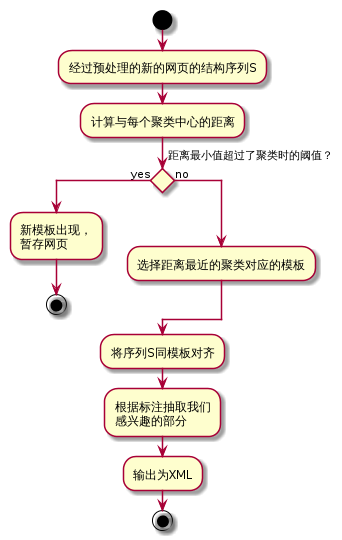
\includegraphics[width=0.5\textwidth]{template05/extractor}
  \caption{内容提取子模块的整体框架}
  \label{template:fig:extractor}
\end{figure}

这里还需要补充两点:第一,由于之前合并了重复记录,因此在提取内容的时候需要进行复
原,将其对应到原网页的多条内容上;第二,对于不属于任何类别的新的模板生成的网页,
我们将其暂存,当其数量到达一定值的时候,我们将用这些网页进行训练,得到新的模板,
加入到现有的系统中,从而实现了新模板的自动识别和生成功能。

\section{本章总结}
\label{sec:summarytemplate}
在这一章中,我们介绍了模板生成和内容提取模块的实现。为了讨论方便,我们首先形式化
地定义了模板,然后我们介绍了如何对每个聚类生成对应的模板,重点在于如何正确构造模
板中的可选节点。最后我们介绍了内容提取模块的具体实现流程。

至此,我们系统的各个模块的具体实现都已经介绍完了。

%%% Local Variables: 
%%% mode: latex
%%% TeX-master: "../main"
%%% End: 


\chapter{系统实现和实验结果}
\label{chap:experiment}

\section{系统具体实现}
\label{sec:implementation}
我们采用Scala语言来搭建我们的系统。Scala是一种运行在JVM上的静态语言,支持函数式、
面向对象等多种编程范式,可以和Java代码无缝地进行交互。目前Scala还处于不断发展中,
新版本不向后兼容,我们的系统在Scala 2.10上可以编译通过。在工程管理上,我们使
用sbt管理Scala代码的编译和依赖关系。

在系统的实现中我们还使用了许多第三方库,除了在第~\ref{chap:cluster}章中介绍
的Actor库Akka,还有:
\begin{itemize}
\item 日志系统:基于twitter公司开源的util包,地址在
  \url{https://github.com/twitter/util}。
\item 网页字符集检测:ICU4J,地址在\url{http://site.icu-project.org},这是一
  套UNICODE相关的工具集,提供了较好的字符集编码检测功能,我们用于检测中文网页的字
  符集。
\item HTML解析器:jsoup,地址在\url{http://jsoup.org},是一个用Java语言实现
  的HTML解析器,用于DOM Tree的构建和节点内容的抽取。
\end{itemize}
\section{模板匹配演示系统}
\label{sec:demo}
为了直观地显示网页模板的匹配效果,我们基于Play! Framework的Web开发框架实现了一
个Web Service,用于实验的演示。该Web Service的工作原理
如\reffig{experiment:fig:demo}所示。
\begin{figure}
  \centering
  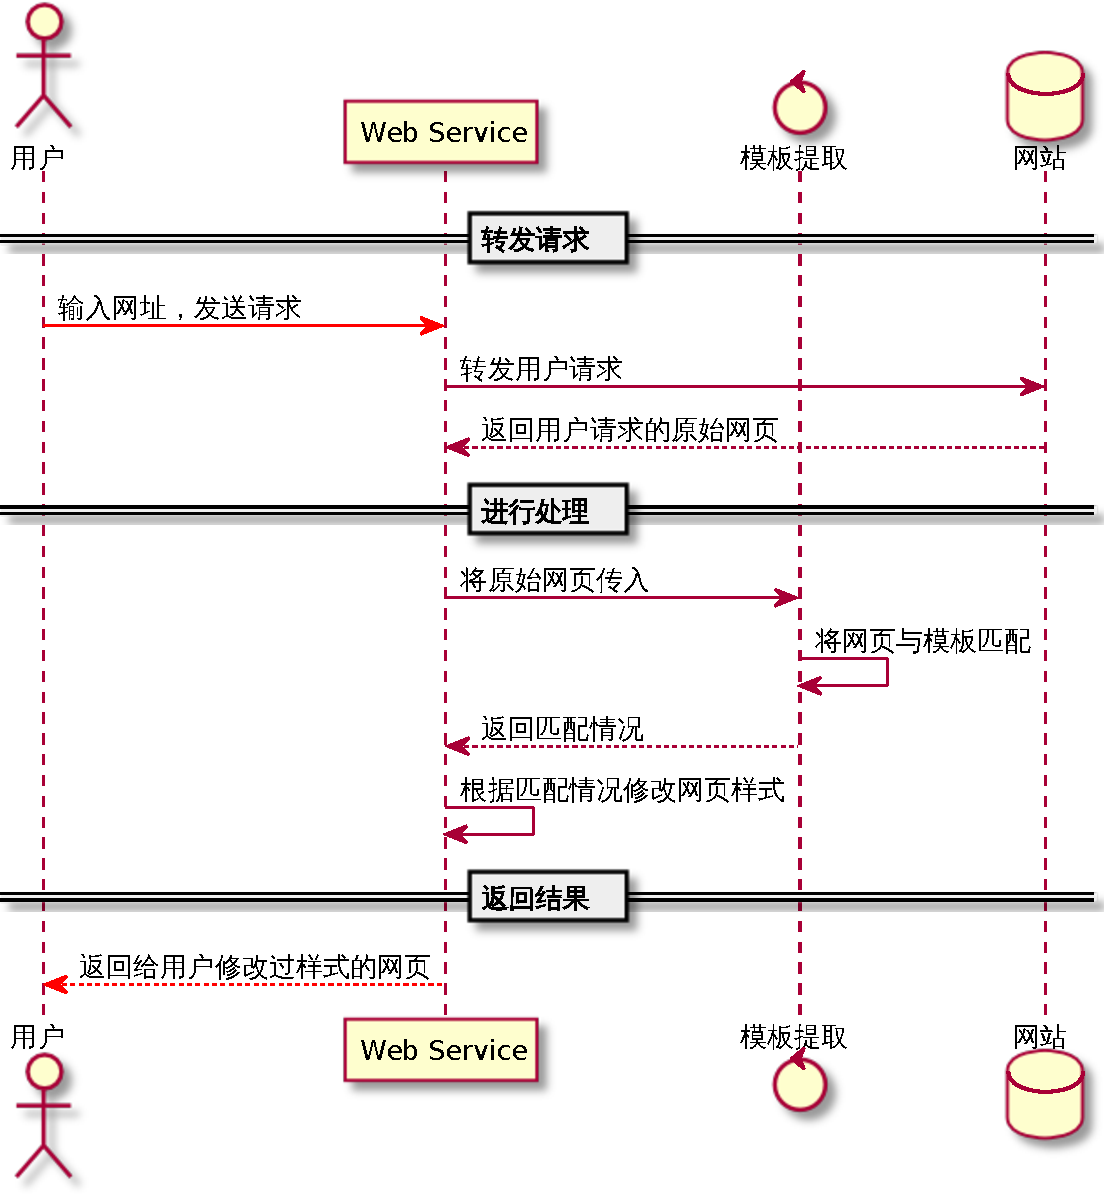
\includegraphics[width=0.75\textwidth]{experiment06/demo}
  \caption{Web Service工作原理}
  \label{experiment:fig:demo}
\end{figure}

用户需要输入一个用于和系统的模板进行匹配的网页的URL,系统返回给用户一个修改了样式
的新的网页,其中原网页和模板匹配上的部分会有和其他部分不同的显示效果,这样用户就
可以通过浏览器中直观地看到模板的匹配效果。

% TODO: 实验演示的效果如\reffig{experiment:fig:demoresult}所示
% \begin{figure}
%   \centering
%   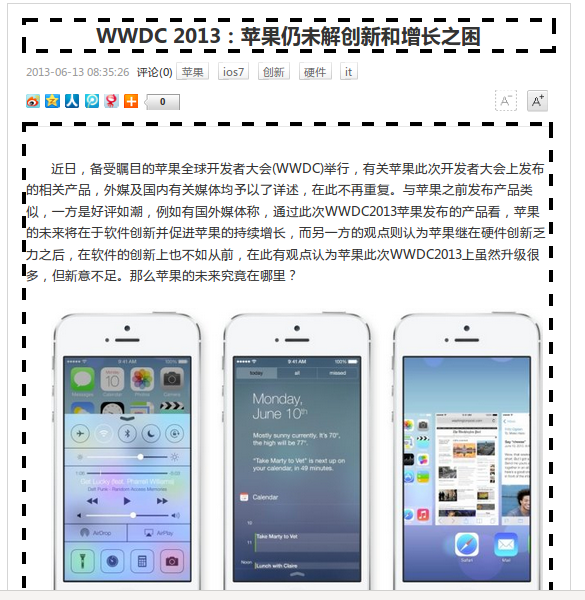
\includegraphics[width=0.5\textwidth]{experiment06/demoresult}
%   \caption{实验演示系统效果}
%   \label{experiment:fig:demoresult}
% \end{figure}

\section{实验和分析}
\label{sec:result-analysis}

\subsection{实验环境和数据}
\label{sec:dataenv}
我们实验所用的机器的配置情况是:16个逻辑核的CPU,24G内存,操作系统为64位的CentOS。
后续的实验均在这个机器上进行。

我们有三个实验数据集,分别为博客(blog),新闻(news)和其他(others)。实验数据
集的概况如\reftbl{experiment:tab:overview}所示。%TODO
\begin{table}[h]
  \centering
% BEGIN RECEIVE ORGTBL 实验数据概况
\begin{tabular}{llll}
\toprule
 & blog & news & other \\
\hline
文件个数 & 59998 & 81561 & 183635 \\
总大小 & 5.4G & 7.9G & 18G \\
来源 & blog.sina.com.cn &  ent.sina.com.cn &  \\
\bottomrule
\end{tabular}
% END RECEIVE ORGTBL 实验数据概况
  \caption{实验数据概况}
  \label{experiment:tab:overview}
\end{table}
\begin{comment}
#+ORGTBL: SEND 实验数据概况 orgtbl-to-latex :splice nil :skip 0
|          | blog             | news            | other  |
|----------+------------------+-----------------+--------|
| 文件个数 | 59998            | 81561           | 183635 |
| 总大小   | 5.4G             | 7.9G            | 18G    |
| 来源     | blog.sina.com.cn | ent.sina.com.cn |        |
\end{comment}

接下来的几个小节我们将大体按照模块的顺序,依次介绍实验的详细情况。
\label{sec:results}
\subsection{预处理模块实验与分析}
\label{sec:experiement:pre}
在预处理模块中,我们首先将从原始的网页集合中过滤掉无用的网页,包括目录页和错误页,
采用的是第~\ref{sec:filterintro-useless}节中介绍的基于规则的方
法。\reftbl{experiment:tab:filter}给出了实验中使用的过滤规则和过滤后的结果。%TODO
\begin{table}[hb]
  \centering
% BEGIN RECEIVE ORGTBL 过滤无用网页
\begin{tabular}{lrrr}
  \toprule
 & blog & news & others \\
\hline
目录页URL规则 & .*(?<!\textbackslash\textbackslash.html?)\$ & .*(?<!\textbackslash\textbackslash.shtml)\$ &  \\
错误页最大长度 & 6000 & 6000 &  \\
文件个数 & 59998 & 81561 & 183635 \\
过滤后详细页个数 &  &  &  \\
\bottomrule
\end{tabular}
% END RECEIVE ORGTBL 过滤无用网页
  \caption{过滤无用网页实验结果}
  \label{experiment:tab:filter}
\end{table}
\begin{comment}
#+ORGTBL: SEND 过滤无用网页 orgtbl-to-latex :splice nil :skip 0
|                  |                                       blog |                                        news | others |
|------------------+--------------------------------------------+---------------------------------------------+--------|
| 目录页URL规则    | .*(?<!\textbackslash\textbackslash.html?)$ | .*(?<!\textbackslash\textbackslash.s?html)$ |        |
| 错误页最大长度   |                                       6000 |                                        6000 |        |
| 原来总文件个数   |                                      59998 |                                       81561 | 183635 |
| 过滤后详细页个数 |                                            |                                       65655 |        |
\end{comment}

过滤掉了不需要的网页以后,我们得到了详细页的集合。在进行下一步的实验之前,我们先
将这些详细页集合分成训练集和测试集,各个数据集的具体分割情况如\reftbl{experiment:tab:split}所示。%TODO
\begin{table}[hb]
\centering
% BEGIN RECEIVE ORGTBL 数据分割
\begin{tabular}{llll}
  \toprule
 & 训练集 & 测试集 & 详细页总数 \\
\hline
blog &  &  &  \\
news &  &  &  \\
others &  &  &  \\
\bottomrule
\end{tabular}
% END RECEIVE ORGTBL 数据分割
\caption{训练集和测试集分布}
\label{experiment:tab:split}
\end{table}
\begin{comment}
#+ORGTBL: SEND 数据分割 orgtbl-to-latex :splice nil :skip 0
|        | 训练集 | 测试集 | 详细页总数 |
|--------+--------+--------+------------|
| blog   |        |        |            |
| news   |        |        |      65655 |
| others |        |        |            |
\end{comment}

接下来将去除无用的标签。\reftbl{experiment:tab:uselesstags}给出了我们实验中去掉无
用标签的几种正则表达式模式及每种模式对应的标签名。
\begin{table}[hb]
  \centering
% BEGIN RECEIVE ORGTBL 无用标签
\begin{tabular}{ll}
  \toprule
正则表达式模式 & 对应的标签名 \\
\hline
(?is)<tag.*?>.*?</tag> & style,script \\
(?is)<[/]?tag.*?> & link,input,br,img,meta,wbr \\
(?is)<[/]?tag.*?> & strong,em,font,b,p,li,ul,ol,td,tr,th,tbody,table \\
\bottomrule
\end{tabular}
% END RECEIVE ORGTBL 无用标签
  \caption{去掉的无用标签}
  \label{experiment:tab:uselesstags}
\end{table}
\begin{comment}
#+ORGTBL: SEND 无用标签 orgtbl-to-latex :splice nil :skip 0
| 正则表达式模式         | 对应的标签名                                     |
|------------------------+--------------------------------------------------|
| (?is)<tag.*?>.*?</tag> | style,script                                     |
| (?is)<[/]?tag.*?>      | link,input,br,img,meta,wbr                       |
| (?is)<[/]?tag.*?>      | strong,em,font,b,p,li,ul,ol,td,tr,th,tbody,table |
\end{comment}

下面我们对利用后缀树检测重复记录的算法的运行结果做一些统计。具体地,我们统计出每
个数据集中算法检测出的重复记录的长度的分布情况,结果如\reffig{experiment:fig:recordlength}所示。% TODO
\begin{figure}[hb]
  \centering
  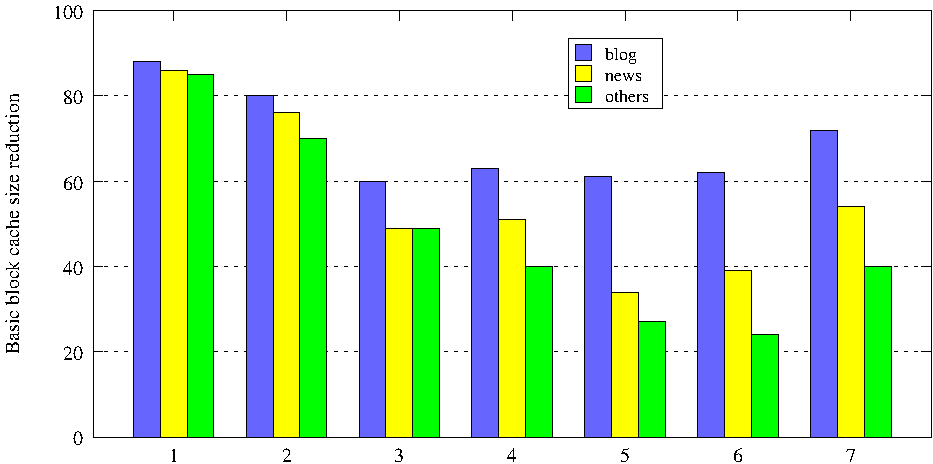
\includegraphics[width=0.8\textwidth]{experiment06/recordlength}
  \caption{检测出的重复记录长度的分布情况}
  \label{experiment:fig:recordlength}
\end{figure}

我们可以看到,大部分的重复记录集中在。% Lorem ipsum dolor sit amet, consectetur adipisicing elit, sed do eiusmod tempor incididunt ut labore et dolore magna aliqua. Ut enimad minim veniam, quis nostrud exercitation ullamco laboris nisi ut aliquip ex ea commodo consequat. Duis aute irure dolor in reprehenderit in voluptate velit esse cillum dolore eu fugiat nulla pariatur. Excepteur sint occaecat cupidatat non proident, sunt in culpa qui officia deserunt mollit anim id est laborum.

\subsection{聚类和模板生成模块实验和分析}
由于我们要处理的网页的数量非常多,计算网页的结构相似度将是我们整个系统最耗时的部
分,因此,我们先将训练集中所有的文档结构相似度离线算好,方便后续的实
验。\reftbl{experiment:tab:calcsim}给出了在各个数据集上计算所有的文档结构相似度的时间统计结果。 % TODO
\begin{table}[h]
  \centering
% BEGIN RECEIVE ORGTBL 计算时间
\begin{tabular}{llll}
  \toprule
 & blog & news & others \\
\hline
训练集大小 &  &  &  \\
所花时间 &  &  &  \\
\bottomrule
\end{tabular}
% END RECEIVE ORGTBL 计算时间
\caption{每个数据集计算全部文档结构相似度的时间}
\label{experiment:tab:calcsim}
\end{table}
\begin{comment}
#+ORGTBL: SEND 计算时间 orgtbl-to-latex :splice nil :skip 0
|            | blog | news | others |
|------------+------+------+--------|
| 训练集大小 |      |      |        |
| 所花时间   |      |      |        |
\end{comment}

可以看到,由于采用了Actor模型进行并行计算%TODO:分析

在聚类模块中,最重要的实验参数是聚类时设置的相似度阈值。为了观察该阈值对实验结果
的影响,我们调整该阈值,观察聚类的个数的变化;同时,我们还将统计根据不同的聚类结
果生成的模块的一些信息,观察聚类阈值的变化对最后模板的生成有怎样的影响。我们选择
在news数据集上进行实验,具体的实验结果见\reftbl{experiment:tab:threshold}。%TODO

\begin{table}
% BEGIN RECEIVE ORGTBL 阈值变化
  \centering
\begin{tabular}{rllll}
  \toprule
阈值 & 聚类个数 & 模板长度 & 必选节点包含的点数 & 可选节点平均长度 \\
\hline
0.2 &  &  &  &  \\
0.3 &  &  &  &  \\
0.4 &  &  &  &  \\
0.5 &  &  &  &  \\
\bottomrule
\end{tabular}
% END RECEIVE ORGTBL 阈值变化
\caption{阈值变化对实验结果的影响\label{experiment:tab:threshold}}
\end{table}
\begin{comment}
#+ORGTBL: SEND 阈值变化 orgtbl-to-latex :splice nil :skip 0
| 阈值 | 聚类个数 | 模板长度 | 必选节点包含的点数 | 可选节点平均长度 |
|------+----------+----------+--------------------+------------------|
|  0.2 |          |          |                    |                  |
|  0.3 |          |          |                    |                  |
|  0.4 |          |          |                    |                  |
|  0.5 |          |          |                    |                  |
\end{comment}


从\reftbl{experiment:tab:threshold}所示的实验结果中,我们可以看到聚类时设置的阈值
大小不仅会影响聚类的个数,对后续的模板生成也有较大的影响。通过分析,我们可以得到以下几个结论:%TODO: 分析!
\begin{itemize}
\item 聚类时的阈值越小,
\end{itemize}

\subsection{内容抽取模块实验}
为了验证我们的系统能在实际的生产环境中使用,我们在测试集上进行了实验。首先是人工
对每个模板进行少量标注,然后利用标注好的模板,对每个新的网页(测试集)进行内容抽
取,最后将抽取的内容用XML格式保存下来。\reffig{experiment:fig:xmloutput}是我们保
存到XML中的结果的截图。
\begin{figure}[hb]
  \centering
  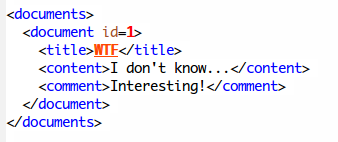
\includegraphics[width=0.5\textwidth]{experiment06/xmloutput}
  \caption{XML保存的结果截图}
  \label{experiment:fig:xmloutput}
\end{figure}

从\reffig{experiment:fig:xmloutput}可以看到,我们。%TODO:
\section{实验结果总结}
\label{sec:analysis}
对于以上的实验结果,我们可以做一个简单的总结:%TODO
\begin{itemize}
\item 在预处理模块
\end{itemize}

%%% Local Variables: 
%%% mode: latex
%%% TeX-master: "../main"
%%% End: 


\chapter{工作总结和未来展望}
\label{chap:future}

\section{工作总结}
\label{sec:summaryall}

\section{未来工作展望}
\label{sec:futurework}

%%% Local Variables: 
%%% mode: latex
%%% TeX-master: "../main"
%%% End: 

% 
%%% Local Variables:
%%% mode: latex
%%% TeX-master: t
%%% End:

\chapter{带 English 的标题}
\label{cha:intro}

这是 \thuthesis{} 的示例文档,基本上覆盖了模板中所有格式的设置。建议大家在使用模
板之前,除了阅读《\thuthesis{}用户手册》,这个示例文档也最好能看一看。

小老鼠偷吃热凉粉;短长虫环绕矮高粱。\footnote{韩愈(768-824),字退之,河南河阳(
  今河南孟县)人,自称郡望昌黎,世称韩昌黎。幼孤贫刻苦好学,德宗贞元八年进士。曾
  任监察御史,因上疏请免关中赋役,贬为阳山县令。后随宰相裴度平定淮西迁刑部侍郎,
  又因上表谏迎佛骨,贬潮州刺史。做过吏部侍郎,死谥文公,故世称韩吏部、韩文公。是
  唐代古文运动领袖,与柳宗元合称韩柳。诗力求险怪新奇,雄浑重气势。}


\section{封面相关}
封面的例子请参看 cover.tex。主要符号表参看 denation.tex,附录和个人简历分别参看 appendix01.tex
和 resume.tex。里面的命令都非常简单,一看即会。\footnote{你说还是看不懂?怎么会呢?}

\section{字体命令}
\label{sec:first}

苏轼(1037-1101),北宋文学家、书画家。字子瞻,号东坡居士,眉州眉山(今属四川)人
。苏洵子。嘉佑进士。神宗时曾任祠部员外郎,因反对王安石新法而求外职,任杭州通判,
知密州、徐州、湖州。后以作诗“谤讪朝廷”罪贬黄州。哲宗时任翰林学士,曾出知杭州、
颖州等,官至礼部尚书。后又贬谪惠州、儋州。北还后第二年病死常州。南宋时追谥文忠。
与父洵弟辙,合称“三苏”。在政治上属于旧党,但也有改革弊政的要求。其文汪洋恣肆,
明白畅达,为“唐宋八大家”之一。  其诗清新豪健,善用夸张比喻,在艺术表现方面独具
风格。少数诗篇也能反映民间疾苦,指责统治者的奢侈骄纵。词开豪放一派,对后代很有影
响。《念奴娇·赤壁怀古》、《水调歌头·丙辰中秋》传诵甚广。

{\kaishu 坡仙擅长行书、楷书,取法李邕、徐浩、颜真卿、杨凝式,而能自创新意。用笔丰腴
  跌宕,有天真烂漫之趣。与蔡襄、黄庭坚、米芾并称“宋四家”。能画竹,学文同,也喜
  作枯木怪石。论画主张“神似”,认为“论画以形似,见与儿童邻”;高度评价“诗中有
  画,画中有诗”的艺术造诣。诗文有《东坡七集》等。存世书迹有《答谢民师论文帖》、
  《祭黄几道文》、《前赤壁赋》、《黄州寒食诗帖》等。  画迹有《枯木怪石图》、《
  竹石图》等。}

{\fangsong 易与天地准,故能弥纶天地之道。仰以观於天文,俯以察於地理,是故知幽明之故。原
  始反终,故知死生之说。精气为物,游魂为变,是故知鬼神之情状。与天地相似,故不违。
  知周乎万物,而道济天下,故不过。旁行而不流,乐天知命,故不忧。安土敦乎仁,故
  能爱。范围天地之化而不过,曲成万物而不遗,通乎昼夜之道而知,故神无方而易无体。}

% 非本科生一般用不到幼圆与隶书字体。ctex 在 xelatex 编译时用 winfonts/adobefonts
% 选项也只配置了四款中文字体,没有提供幼圆和隶书。需要的同学可以使用 nofonts 选项
% 自行配置中文字体,或者换用 pdflatex 引擎编译。
{\ifcsname youyuan\endcsname\youyuan 有天地,然后万物生焉。盈天地之间者,唯万物,故受之以屯;屯者盈也,屯者物之
  始生也。物生必蒙,故受之以蒙;蒙者蒙也,物之穉也。物穉不可不养也,故受之以需;
  需者饮食之道也。饮食必有讼,故受之以讼。讼必有众起,故受之以师;师者众也。众必
  有所比,故受之以比;比者比也。比必有所畜也,故受之以小畜。物畜然后有礼,故受之
  以履。\fi}

{\heiti 履而泰,然后安,故受之以泰;泰者通也。物不可以终通,故受之以否。物不可以终
  否,故受之以同人。与人同者,物必归焉,故受之以大有。有大者不可以盈,故受之以谦。
  有大而能谦,必豫,故受之以豫。豫必有随,故受之以随。以喜随人者,必有事,故受
  之以蛊;蛊者事也。}

{\ifcsname lishu\endcsname\lishu 有事而后可大,故受之以临;临者大也。物大然后可观,故受之以观。可观而后有所合
  ,故受之以噬嗑;嗑者合也。物不可以苟合而已,故受之以贲;贲者饰也。致饰然后亨
  ,则尽矣,故受之以剥;剥者剥也。物不可以终尽,剥穷上反下,故受之以复。复则不
  妄矣,故受之以无妄。\fi}

{\songti 有无妄然后可畜,故受之以大畜。物畜然后可养,故受之以颐;颐者养也。不养则不
  可动,故受之以大过。物不可以终过,故受之以坎;坎者陷也。陷必有所丽,故受之以
  离;离者丽也。}

\section{表格样本}
\label{chap1:sample:table} 

\subsection{基本表格}
\label{sec:basictable}

模板中关于表格的宏包有三个: \textsf{booktabs}、\textsf{array} 和
\textsf{longtabular},命令有一个 \verb|\hlinewd|。三线表可以用 \textsf{booktabs}
提供的 \verb|\toprule|、\verb|\midrule| 和 \verb|\bottomrule|。它们与
\textsf{longtable} 能很好的配合使用。如果表格比较简单的话可以直接用命令
\verb|hlinewd{xpt}| 控制。
\begin{table}[htb]
  \centering
  \begin{minipage}[t]{0.8\linewidth} % 如果想在表格中使用脚注,minipage是个不错的办法
  \caption[模板文件]{模板文件。如果表格的标题很长,那么在表格索引中就会很不美
    观,所以要像 chapter 那样在前面用中括号写一个简短的标题。这个标题会出现在索
    引中。}
  \label{tab:template-files}
    \begin{tabular*}{\linewidth}{lp{10cm}}
      \toprule[1.5pt]
      {\heiti 文件名} & {\heiti 描述} \\\midrule[1pt]
      thuthesis.ins & \LaTeX{} 安装文件,docstrip\footnote{表格中的脚注} \\
      thuthesis.dtx & 所有的一切都在这里面\footnote{再来一个}。\\
      thuthesis.cls & 模板类文件。\\
      thuthesis.cfg & 模板配置文。cls 和 cfg 由前两个文件生成。\\
      thubib.bst    & 参考文献 Bibtex 样式文件。\\
      thutils.sty   & 常用的包和命令写在这里,减轻主文件的负担。\\
      \bottomrule[1.5pt]
    \end{tabular*}
  \end{minipage}
\end{table}

首先来看一个最简单的表格。表 \ref{tab:template-files} 列举了本模板主要文件及其功
能。请大家注意三线表中各条线对应的命令。这个例子还展示了如何在表格中正确使用脚注。
由于 \LaTeX{} 本身不支持在表格中使用 \verb|\footnote|,所以我们不得不将表格放在
小页中,而且最好将表格的宽度设置为小页的宽度,这样脚注看起来才更美观。

\subsection{复杂表格}
\label{sec:complicatedtable}

我们经常会在表格下方标注数据来源,或者对表格里面的条目进行解释。前面的脚注是一种
不错的方法,如果你不喜欢脚注。那么完全可以在表格后面自己写注释,比如表~\ref{tab:tabexamp1}。
\begin{table}[htbp]
  \centering
  \caption{复杂表格示例 1}
  \label{tab:tabexamp1}
  \begin{minipage}[t]{0.8\textwidth} 
    \begin{tabularx}{\linewidth}{|l|X|X|X|X|}
      \hline
 \multirow{2}*{\diagbox[width=5em]{x}{y}}  & \multicolumn{2}{c|}{First Half} & \multicolumn{2}{c|}{Second Half}\\\cline{2-5}
      & 1st Qtr &2nd Qtr&3rd Qtr&4th Qtr \\ \hline
      East$^{*}$ &   20.4&   27.4&   90&     20.4 \\
      West$^{**}$ &   30.6 &   38.6 &   34.6 &  31.6 \\ \hline
    \end{tabularx}\\[2pt]
    \footnotesize 注:数据来源《\thuthesis{} 使用手册》。\\
    *:东部\\
    **:西部
  \end{minipage}
\end{table}

此外,表~\ref{tab:tabexamp1} 同时还演示了另外两个功能:1)通过 \textsf{tabularx} 的
 \texttt{|X|} 扩展实现表格自动放大;2)通过命令 \verb|\diagbox| 在表头部分
插入反斜线。

为了使我们的例子更接近实际情况,我会在必要的时候插入一些“无关”文字,以免太多图
表同时出现,导致排版效果不太理想。第一个出场的当然是我的最爱:风流潇洒、骏马绝尘、
健笔凌云的{\heiti 李太白}了。

李白,字太白,陇西成纪人。凉武昭王暠九世孙。或曰山东人,或曰蜀人。白少有逸才,志
气宏放,飘然有超世之心。初隐岷山,益州长史苏颋见而异之,曰:“是子天才英特,可比
相如。”天宝初,至长安,往见贺知章。知章见其文,叹曰:“子谪仙人也。”言于明皇,
召见金銮殿,奏颂一篇。帝赐食,亲为调羹,有诏供奉翰林。白犹与酒徒饮于市,帝坐沉香
亭子,意有所感,欲得白为乐章,召入,而白已醉。左右以水颒面,稍解,援笔成文,婉丽
精切。帝爱其才,数宴见。白常侍帝,醉,使高力士脱靴。力士素贵,耻之,摘其诗以激杨
贵妃。帝欲官白,妃辄沮止。白自知不为亲近所容,恳求还山。帝赐金放还。乃浪迹江湖,
终日沉饮。永王璘都督江陵,辟为僚佐。璘谋乱,兵败,白坐长流夜郎,会赦得还。族人阳
冰为当涂令,白往依之。代宗立,以左拾遗召,而白已卒。文宗时,诏以白歌诗、裴旻剑舞、
张旭草书为三绝云。集三十卷。今编诗二十五卷。\hfill\pozhehao《全唐诗》诗人小传

浮动体的并排放置一般有两种情况:1)二者没有关系,为两个独立的浮动体;2)二者隶属
于同一个浮动体。对表格来说并排表格既可以像图~\ref{tab:parallel1}、图~\ref{tab:parallel2} 
使用小页环境,也可以如图~\ref{tab:subtable} 使用子表格来做。图的例子参见第~\ref{sec:multifig} 节。
\begin{table}[htbp]
\noindent\begin{minipage}{0.5\textwidth}
\centering
\caption{第一个并排子表格}
\label{tab:parallel1}
\begin{tabular}{p{2cm}p{2cm}}
\toprule[1.5pt]
111 & 222 \\\midrule[1pt]
222 & 333 \\\bottomrule[1.5pt]
\end{tabular}
\end{minipage}
\begin{minipage}{0.5\textwidth}
\centering
\caption{第二个并排子表格}
\label{tab:parallel2}
\begin{tabular}{p{2cm}p{2cm}}
\toprule[1.5pt]
111 & 222 \\\midrule[1pt]
222 & 333 \\\bottomrule[1.5pt]
\end{tabular}
\end{minipage}
\end{table}

然后就是忧国忧民,诗家楷模杜工部了。杜甫,字子美,其先襄阳人,曾祖依艺为巩令,因
居巩。甫天宝初应进士,不第。后献《三大礼赋》,明皇奇之,召试文章,授京兆府兵曹参
军。安禄山陷京师,肃宗即位灵武,甫自贼中遁赴行在,拜左拾遗。以论救房琯,出为华州
司功参军。关辅饥乱,寓居同州同谷县,身自负薪采梠,餔糒不给。久之,召补京兆府功曹,
道阻不赴。严武镇成都,奏为参谋、检校工部员外郎,赐绯。武与甫世旧,待遇甚厚。乃于
成都浣花里种竹植树,枕江结庐,纵酒啸歌其中。武卒,甫无所依,乃之东蜀就高適。既至
而適卒。是岁,蜀帅相攻杀,蜀大扰。甫携家避乱荆楚,扁舟下峡,未维舟而江陵亦乱。乃
溯沿湘流,游衡山,寓居耒阳。卒年五十九。元和中,归葬偃师首阳山,元稹志其墓。天宝
间,甫与李白齐名,时称李杜。然元稹之言曰:“李白壮浪纵恣,摆去拘束,诚亦差肩子美
矣。至若铺陈终始,排比声韵,大或千言,次犹数百,词气豪迈,而风调清深,属对律切,
而脱弃凡近,则李尚不能历其藩翰,况堂奥乎。”白居易亦云:“杜诗贯穿古今,  尽工尽
善,殆过于李。”元、白之论如此。盖其出处劳佚,喜乐悲愤,好贤恶恶,一见之于诗。而
又以忠君忧国、伤时念乱为本旨。读其诗可以知其世,故当时谓之“诗史”。旧集诗文共六
十卷,今编诗十九卷。

\begin{table}[htbp]
\centering
\caption{并排子表格}
\label{tab:subtable}
\subcaptionbox{第一个子表格}
{
\begin{tabular}{p{2cm}p{2cm}}
\toprule[1.5pt]
111 & 222 \\\midrule[1pt]
222 & 333 \\\bottomrule[1.5pt]
\end{tabular}
}
\hskip2cm
\subcaptionbox{第二个子表格}
{
\begin{tabular}{p{2cm}p{2cm}}
\toprule[1.5pt]
111 & 222 \\\midrule[1pt]
222 & 333 \\\bottomrule[1.5pt]
\end{tabular}
}
\end{table}

不可否认 \LaTeX{} 的表格功能没有想象中的那么强大,不过只要你足够认真,足够细致,那么
同样可以排出来非常复杂非常漂亮的表格。请参看表~\ref{tab:tabexamp2}。
\begin{table}[htbp]
  \centering\dawu[1.3]
  \caption{复杂表格示例 2}
  \label{tab:tabexamp2}
  \begin{tabular}[c]{|c|m{0.8in}|c|c|c|c|c|}\hline
    \multicolumn{2}{|c|}{Network Topology} & \# of nodes & 
    \multicolumn{3}{c|}{\# of clients} & Server \\\hline
    GT-ITM & Waxman Transit-Stub & 600 &
    \multirow{2}{2em}{2\%}& 
    \multirow{2}{2em}{10\%}& 
    \multirow{2}{2em}{50\%}& 
    \multirow{2}{1.2in}{Max. Connectivity}\\\cline{1-3}
    \multicolumn{2}{|c|}{Inet-2.1} & 6000 & & & &\\\hline
    \multirow{2}{1in}{Xue} & Rui  & Ni &\multicolumn{4}{c|}{\multirow{2}*{\thuthesis}}\\\cline{2-3}
    & \multicolumn{2}{c|}{ABCDEF} &\multicolumn{4}{c|}{} \\\hline
\end{tabular}
\end{table}

最后就是清新飘逸、文约意赅、空谷绝响的王大侠了。王维,字摩诘,河东人。工书画,与
弟缙俱有俊才。开元九年,进士擢第,调太乐丞。坐累为济州司仓参军,历右拾遗、监察御
史、左补阙、库部郎中,拜吏部郎中。天宝末,为给事中。安禄山陷两都,维为贼所得,服
药阳喑,拘于菩提寺。禄山宴凝碧池,维潜赋诗悲悼,闻于行在。贼平,陷贼官三等定罪,
特原之,责授太子中允,迁中庶子、中书舍人。复拜给事中,转尚书右丞。维以诗名盛于开
元、天宝间,宁薛诸王驸马豪贵之门,无不拂席迎之。得宋之问辋川别墅,山水绝胜,与道
友裴迪,浮舟往来,弹琴赋诗,啸咏终日。笃于奉佛,晚年长斋禅诵。一日,忽索笔作书
数纸,别弟缙及平生亲故,舍笔而卒。赠秘书监。宝应中,代宗问缙:“朕常于诸王坐闻维
乐章,今存几何?”缙集诗六卷,文四卷,表上之。敕答云,卿伯氏位列先朝,名高希代。
抗行周雅,长揖楚辞。诗家者流,时论归美。克成编录,叹息良深。殷璠谓维诗词秀调雅,
意新理惬。在泉成珠,著壁成绘。苏轼亦云:“维诗中有画,画中有诗也。”今编诗四卷。

要想用好论文模板还是得提前学习一些 \TeX/\LaTeX{}的相关知识,具备一些基本能力,掌
握一些常见技巧,否则一旦遇到问题还真是比较麻烦。我们见过很多这样的同学,一直以来
都是使用 Word 等字处理工具,以为 \LaTeX{}模板的用法也应该类似,所以就沿袭同样的思
路来对待这种所见非所得的排版工具,结果被折腾的焦头烂额,疲惫不堪。

如果您要排版的表格长度超过一页,那么推荐使用 \textsf{longtable} 或者 \textsf{supertabular} 
宏包,模板对 \textsf{longtable} 进行了相应的设置,所以用起来可能简单一些。
表~\ref{tab:performance} 就是 \textsf{longtable} 的简单示例。
\begin{longtable}[c]{c*{6}{r}}
\caption{实验数据}\label{tab:performance}\\
\toprule[1.5pt]
 测试程序 & \multicolumn{1}{c}{正常运行} & \multicolumn{1}{c}{同步} & \multicolumn{1}{c}{检查点} & \multicolumn{1}{c}{卷回恢复}
& \multicolumn{1}{c}{进程迁移} & \multicolumn{1}{c}{检查点} \\
& \multicolumn{1}{c}{时间 (s)}& \multicolumn{1}{c}{时间 (s)}&
\multicolumn{1}{c}{时间 (s)}& \multicolumn{1}{c}{时间 (s)}& \multicolumn{1}{c}{
  时间 (s)}&  文件(KB)\\\midrule[1pt]
\endfirsthead
\multicolumn{7}{c}{续表~\thetable\hskip1em 实验数据}\\
\toprule[1.5pt]
 测试程序 & \multicolumn{1}{c}{正常运行} & \multicolumn{1}{c}{同步} & \multicolumn{1}{c}{检查点} & \multicolumn{1}{c}{卷回恢复}
& \multicolumn{1}{c}{进程迁移} & \multicolumn{1}{c}{检查点} \\
& \multicolumn{1}{c}{时间 (s)}& \multicolumn{1}{c}{时间 (s)}&
\multicolumn{1}{c}{时间 (s)}& \multicolumn{1}{c}{时间 (s)}& \multicolumn{1}{c}{
  时间 (s)}&  文件(KB)\\\midrule[1pt]
\endhead
\hline
\multicolumn{7}{r}{续下页}
\endfoot
\endlastfoot
CG.A.2 & 23.05 & 0.002 & 0.116 & 0.035 & 0.589 & 32491 \\
CG.A.4 & 15.06 & 0.003 & 0.067 & 0.021 & 0.351 & 18211 \\
CG.A.8 & 13.38 & 0.004 & 0.072 & 0.023 & 0.210 & 9890 \\
CG.B.2 & 867.45 & 0.002 & 0.864 & 0.232 & 3.256 & 228562 \\
CG.B.4 & 501.61 & 0.003 & 0.438 & 0.136 & 2.075 & 123862 \\
CG.B.8 & 384.65 & 0.004 & 0.457 & 0.108 & 1.235 & 63777 \\
MG.A.2 & 112.27 & 0.002 & 0.846 & 0.237 & 3.930 & 236473 \\
MG.A.4 & 59.84 & 0.003 & 0.442 & 0.128 & 2.070 & 123875 \\
MG.A.8 & 31.38 & 0.003 & 0.476 & 0.114 & 1.041 & 60627 \\
MG.B.2 & 526.28 & 0.002 & 0.821 & 0.238 & 4.176 & 236635 \\
MG.B.4 & 280.11 & 0.003 & 0.432 & 0.130 & 1.706 & 123793 \\
MG.B.8 & 148.29 & 0.003 & 0.442 & 0.116 & 0.893 & 60600 \\
LU.A.2 & 2116.54 & 0.002 & 0.110 & 0.030 & 0.532 & 28754 \\
LU.A.4 & 1102.50 & 0.002 & 0.069 & 0.017 & 0.255 & 14915 \\
LU.A.8 & 574.47 & 0.003 & 0.067 & 0.016 & 0.192 & 8655 \\
LU.B.2 & 9712.87 & 0.002 & 0.357 & 0.104 & 1.734 & 101975 \\
LU.B.4 & 4757.80 & 0.003 & 0.190 & 0.056 & 0.808 & 53522 \\
LU.B.8 & 2444.05 & 0.004 & 0.222 & 0.057 & 0.548 & 30134 \\
EP.A.2 & 123.81 & 0.002 & 0.010 & 0.003 & 0.074 & 1834 \\
EP.A.4 & 61.92 & 0.003 & 0.011 & 0.004 & 0.073 & 1743 \\
EP.A.8 & 31.06 & 0.004 & 0.017 & 0.005 & 0.073 & 1661 \\
EP.B.2 & 495.49 & 0.001 & 0.009 & 0.003 & 0.196 & 2011 \\
EP.B.4 & 247.69 & 0.002 & 0.012 & 0.004 & 0.122 & 1663 \\
EP.B.8 & 126.74 & 0.003 & 0.017 & 0.005 & 0.083 & 1656 \\
\bottomrule[1.5pt]
\end{longtable}

\subsection{其它}
\label{sec:tableother}
有的同学不想让某个表格或者图片出现在索引里面,那么请使用命令 \verb|\caption*{}|,
这个命令不会给表格编号,也就是出来的只有标题文字而没有“表~XX”,“图~XX”,否则
索引里面序号不连续就显得不伦不类,这也是 \LaTeX{} 里星号命令默认的规则。

有这种需求的多是本科同学的英文资料翻译部分,如果你觉得附录中英文原文中的表格和图
片显示成“  表”和“图”很不协调的话,一个很好的办法就是用 \verb|\caption*|,参数
随便自己写,比如不守规矩的表~1.111 和图~1.111 能满足这种特殊需要(可以参看附录部
分)。
\begin{table}[ht]
\centering
  \begin{minipage}{0.45\linewidth}
  \centering
  \caption*{表~1.111\hskip1em 这是一个手动编号,不出现在索引中的表格。}
  \label{tab:badtabular}
  \begin{picture}(150,50)
    \framebox(150,50)[c]{\thuthesis}
  \end{picture}    
  \end{minipage}\hfill
  \begin{minipage}{0.45\linewidth}
  \centering
  \begin{picture}(150,50)
    \framebox(150,50)[c]{薛瑞尼}
  \end{picture}
  \caption*{Figure~1.111\hskip1em 这是一个手动编号,不出现在索引中的图。}
  \label{tab:badfigure}
  \end{minipage}
\end{table}

如果你的确想让它编号,但又不想让它出现在索引中的话,那就自己看看代码改一改吧,我
目前不打算给模板增加这种另类命令。

最后,虽然大家不一定会独立使用小页,但是关于小页中的脚注还是有必要提一下。请看下
面的例子。

\begin{minipage}[t]{\linewidth-2\parindent}
  柳宗元,字子厚(773-819),河东(今永济县)人\footnote{山西永济水饺。},是唐代
  杰出的文学家,哲学家,同时也是一位政治改革家。与韩愈共同倡导唐代古文运动,并称
  韩柳\footnote{唐宋八大家之首二位。}。
\end{minipage}\\[-5pt]

唐朝安史之乱后,宦官专权,藩镇割据,土地兼并日渐严重,社会生产破坏严重,民不聊生。柳宗
元对这种社会现实极为不满,他积极参加了王叔文领导的“永济革新”,并成为这一
运动的中坚人物。他们革除弊政,打击权奸,触犯了宦官和官僚贵族利益,在他们的联合反
扑下,改革失败了,柳宗元被贬为永州司马。

\section{定理环境}
\label{sec:theorem}

给大家演示一下各种和证明有关的环境:

\begin{assumption}
待月西厢下,迎风户半开;隔墙花影动,疑是玉人来。
\begin{eqnarray}
  \label{eq:eqnxmp}
  c & = & a^2 - b^2\\
    & = & (a+b)(a-b)
\end{eqnarray}
\end{assumption}

千辛万苦,历尽艰难,得有今日。然相从数千里,未曾哀戚。今将渡江,方图百年欢笑,如
何反起悲伤?(引自《杜十娘怒沉百宝箱》)

\begin{definition}
子曰:「道千乘之国,敬事而信,节用而爱人,使民以时。」
\end{definition}

千古第一定义!问世间、情为何物,只教生死相许?天南地北双飞客,老翅几回寒暑。欢乐趣,离别苦,就中更有痴儿女。
君应有语,渺万里层云,千山暮雪,只影向谁去?

横汾路,寂寞当年箫鼓,荒烟依旧平楚。招魂楚些何嗟及,山鬼暗谛风雨。天也妒,未信与,莺儿燕子俱黄土。
千秋万古,为留待骚人,狂歌痛饮,来访雁丘处。

\begin{proposition}
 曾子曰:「吾日三省吾身 \pozhehao 为人谋而不忠乎?与朋友交而不信乎?传不习乎?」
\end{proposition}

多么凄美的命题啊!其日牛马嘶,新妇入青庐,奄奄黄昏后,寂寂人定初,我命绝今日,
魂去尸长留,揽裙脱丝履,举身赴清池,府吏闻此事,心知长别离,徘徊庭树下,自挂东南
枝。

\begin{remark}
天不言自高,水不言自流。
\begin{gather*}
\begin{split} 
\varphi(x,z)
&=z-\gamma_{10}x-\gamma_{mn}x^mz^n\\
&=z-Mr^{-1}x-Mr^{-(m+n)}x^mz^n
\end{split}\\[6pt]
\begin{align} \zeta^0&=(\xi^0)^2,\\
\zeta^1 &=\xi^0\xi^1,\\
\zeta^2 &=(\xi^1)^2,
\end{align}
\end{gather*}
\end{remark}

天尊地卑,乾坤定矣。卑高以陈,贵贱位矣。 动静有常,刚柔断矣。方以类聚,物以群分,
吉凶生矣。在天成象,在地成形,变化见矣。鼓之以雷霆,润之以风雨,日月运行,一寒一
暑,乾道成男,坤道成女。乾知大始,坤作成物。乾以易知,坤以简能。易则易知,简则易
从。易知则有亲,易从则有功。有亲则可久,有功则可大。可久则贤人之德,可大则贤人之
业。易简,而天下矣之理矣;天下之理得,而成位乎其中矣。

\begin{axiom}
两点间直线段距离最短。  
\begin{align}
x&\equiv y+1\pmod{m^2}\\
x&\equiv y+1\mod{m^2}\\
x&\equiv y+1\pod{m^2}
\end{align}
\end{axiom}

《彖曰》:大哉乾元,万物资始,乃统天。云行雨施,品物流形。大明始终,六位时成,时
乘六龙以御天。乾道变化,各正性命,保合大和,乃利贞。首出庶物,万国咸宁。

《象曰》:天行健,君子以自强不息。潜龙勿用,阳在下也。见龙再田,德施普也。终日乾
乾,反复道也。或跃在渊,进无咎也。飞龙在天,大人造也。亢龙有悔,盈不可久也。用九,
天德不可为首也。   

\begin{lemma}
《猫和老鼠》是我最爱看的动画片。
\begin{multline*}%\tag*{[a]} % 这个不出现在索引中
\int_a^b\biggl\{\int_a^b[f(x)^2g(y)^2+f(y)^2g(x)^2]
 -2f(x)g(x)f(y)g(y)\,dx\biggr\}\,dy \\
 =\int_a^b\biggl\{g(y)^2\int_a^bf^2+f(y)^2
  \int_a^b g^2-2f(y)g(y)\int_a^b fg\biggr\}\,dy
\end{multline*}
\end{lemma}

行行重行行,与君生别离。相去万余里,各在天一涯。道路阻且长,会面安可知。胡马依北
风,越鸟巢南枝。相去日已远,衣带日已缓。浮云蔽白日,游子不顾返。思君令人老,岁月
忽已晚。  弃捐勿复道,努力加餐饭。

\begin{theorem}\label{the:theorem1}
犯我强汉者,虽远必诛\hfill \pozhehao 陈汤(汉)
\end{theorem}
\begin{subequations}
\begin{align}
y & = 1 \\
y & = 0
\end{align}
\end{subequations}
道可道,非常道。名可名,非常名。无名天地之始;有名万物之母。故常无,欲以观其妙;
常有,欲以观其徼。此两者,同出而异名,同谓之玄。玄之又玄,众妙之门。上善若水。水
善利万物而不争,处众人之所恶,故几于道。曲则全,枉则直,洼则盈,敝则新,少则多,
多则惑。人法地,地法天,天法道,道法自然。知人者智,自知者明。胜人者有力,自胜
者强。知足者富。强行者有志。不失其所者久。死而不亡者寿。

\begin{proof}
燕赵古称多感慨悲歌之士。董生举进士,连不得志于有司,怀抱利器,郁郁适兹土,吾
知其必有合也。董生勉乎哉?

夫以子之不遇时,苟慕义强仁者,皆爱惜焉,矧燕、赵之士出乎其性者哉!然吾尝闻
风俗与化移易,吾恶知其今不异于古所云邪?聊以吾子之行卜之也。董生勉乎哉?

吾因子有所感矣。为我吊望诸君之墓,而观于其市,复有昔时屠狗者乎?为我谢
曰:“明天子在上,可以出而仕矣!” \hfill\pozhehao 韩愈《送董邵南序》
\end{proof}

\begin{corollary}
  四川话配音的《猫和老鼠》是世界上最好看最好听最有趣的动画片。
\begin{alignat}{3}
V_i & =v_i - q_i v_j, & \qquad X_i & = x_i - q_i x_j,
 & \qquad U_i & = u_i,
 \qquad \text{for $i\ne j$;}\label{eq:B}\\
V_j & = v_j, & \qquad X_j & = x_j,
  & \qquad U_j & u_j + \sum_{i\ne j} q_i u_i.
\end{alignat}
\end{corollary}

迢迢牵牛星,皎皎河汉女。
纤纤擢素手,札札弄机杼。
终日不成章,泣涕零如雨。
河汉清且浅,相去复几许。
盈盈一水间,脉脉不得语。

\begin{example}
  大家来看这个例子。
\begin{equation}
\label{ktc}
\left\{\begin{array}{l}
\nabla f({\mbox{\boldmath $x$}}^*)-\sum\limits_{j=1}^p\lambda_j\nabla g_j({\mbox{\boldmath $x$}}^*)=0\\[0.3cm]
\lambda_jg_j({\mbox{\boldmath $x$}}^*)=0,\quad j=1,2,\cdots,p\\[0.2cm]
\lambda_j\ge 0,\quad j=1,2,\cdots,p.
\end{array}\right.
\end{equation}
\end{example}

\begin{exercise}
  清列出 Andrew S. Tanenbaum 和 W. Richard Stevens 的所有著作。
\end{exercise}

\begin{conjecture} \textit{Poincare Conjecture} If in a closed three-dimensional
  space, any closed curves can shrink to a point continuously, this space can be
  deformed to a sphere.
\end{conjecture}

\begin{problem}
 回答还是不回答,是个问题。 
\end{problem}

如何引用定理~\ref{the:theorem1} 呢?加上 \verb|label| 使用 \verb|ref| 即可。妾发
初覆额,折花门前剧。郎骑竹马来,绕床弄青梅。同居长干里,两小无嫌猜。 十四为君妇,
羞颜未尝开。低头向暗壁,千唤不一回。十五始展眉,愿同尘与灰。常存抱柱信,岂上望夫
台。 十六君远行,瞿塘滟滪堆。五月不可触,猿声天上哀。门前迟行迹,一一生绿苔。苔深
不能扫,落叶秋风早。八月蝴蝶来,双飞西园草。感此伤妾心,坐愁红颜老。

\section{参考文献}
\label{sec:bib}
当然参考文献可以直接写 bibitem,虽然费点功夫,但是好控制,各种格式可以自己随意改
写。

本模板推荐使用 BIB\TeX,样式文件为 thubib.bst,基本符合学校的参考文献格式(如专利
等引用未加详细测试)。看看这个例子,关于书的\cite{tex, companion, ColdSources},
还有这些\cite{Krasnogor2004e, clzs, zjsw},关于杂志的\cite{ELIDRISSI94,
  MELLINGER96, SHELL02},硕士论文\cite{zhubajie, metamori2004},博士论文
\cite{shaheshang, FistSystem01},标准文件\cite{IEEE-1363},会议论文\cite{DPMG,kocher99},技术报告\cite{NPB2}。中文参
考文献\cite{cnarticle}应增加 \texttt{lang=``zh''} 字段,以便进行相应处理。另
外,这个 bst 对中文文献\cite{cnproceed}的支持并不是十全十美,如果有不如意的地方,
请手动修改 bbl 文件。

有时候不想要上标,那么可以这样 \onlinecite{shaheshang},这个非常重要。

\section{公式}
\label{sec:equation}
贝叶斯公式如式~(\ref{equ:chap1:bayes}),其中 $p(y|\mathbf{x})$ 为后验;
$p(\mathbf{x})$ 为先验;分母 $p(\mathbf{x})$ 为归一化因子。
\begin{equation}
\label{equ:chap1:bayes}
p(y|\mathbf{x}) = \frac{p(\mathbf{x},y)}{p(\mathbf{x})}=
\frac{p(\mathbf{x}|y)p(y)}{p(\mathbf{x})} 
\end{equation}

论文里面公式越多,\TeX{} 就越 happy。再看一个 \textsf{amsmath} 的例子:
\newcommand{\envert}[1]{\left\lvert#1\right\rvert} 
\begin{equation}\label{detK2}
\det\mathbf{K}(t=1,t_1,\dots,t_n)=\sum_{I\in\mathbf{n}}(-1)^{\envert{I}}
\prod_{i\in I}t_i\prod_{j\in I}(D_j+\lambda_jt_j)\det\mathbf{A}
^{(\lambda)}(\overline{I}|\overline{I})=0.
\end{equation} 

前面定理示例部分列举了很多公式环境,可以说把常见的情况都覆盖了,大家在写公式的时
候一定要好好看 \textsf{amsmath} 的文档,并参考模板中的用法:
\begin{multline*}%\tag{[b]} % 这个出现在索引中的
\int_a^b\biggl\{\int_a^b[f(x)^2g(y)^2+f(y)^2g(x)^2]
 -2f(x)g(x)f(y)g(y)\,dx\biggr\}\,dy \\
 =\int_a^b\biggl\{g(y)^2\int_a^bf^2+f(y)^2
  \int_a^b g^2-2f(y)g(y)\int_a^b fg\biggr\}\,dy
\end{multline*}

其实还可以看看这个多级规划:
\begin{equation}\label{bilevel}
\left\{\begin{array}{l}
\max\limits_{{\mbox{\footnotesize\boldmath $x$}}} F(x,y_1^*,y_2^*,\cdots,y_m^*)\\[0.2cm]
\mbox{subject to:}\\[0.1cm]
\qquad G(x)\le 0\\[0.1cm]
\qquad(y_1^*,y_2^*,\cdots,y_m^*)\mbox{ solves problems }(i=1,2,\cdots,m)\\[0.1cm]
\qquad\left\{\begin{array}{l}
    \max\limits_{{\mbox{\footnotesize\boldmath $y_i$}}}f_i(x,y_1,y_2,\cdots,y_m)\\[0.2cm]
    \mbox{subject to:}\\[0.1cm]
    \qquad g_i(x,y_1,y_2,\cdots,y_m)\le 0.
    \end{array}\right.
\end{array}\right.
\end{equation}
这些跟规划相关的公式都来自于刘宝碇老师《不确定规划》的课件。

\section{破折号}
\label{sec:pozhehao}

中文破折号为一个两个字宽垂直居中的直线,输入法直接得到的破折号是两个断开的小短线
(——),这看起来不舒服。所以我定义了一个破折号的命令 \verb|\pozhehao|,请看几个
例子:
\begin{itemize}
\item 这是一个 \pozhehao 破折号
  \begin{enumerate}[(1)]
  \item 同时也可以看看
  \item 不同列表环境的间距
  \end{enumerate}
\item 看起来这个要好一些
\item 破折号 \pozhehao 就说到这里。
\end{itemize}

默认的列表环境上下间距很大,模板将其重定义为 \textsf{paralist} 中的压缩环境,看起
来要好一些。如果还是不满意,自己也可以调 \verb|\itemsep| 的。\textsf{paralist} 还
可以方便的指定标签的样式。


% 
%%% Local Variables: 
%%% mode: latex
%%% TeX-master: t
%%% End: 

\chapter{中华人民共和国}
\label{cha:china}

\section{其它例子}
\label{sec:other}

在第~\ref{cha:intro} 章中我们学习了贝叶斯公式~(\ref{equ:chap1:bayes}),这里我们复
习一下:
\begin{equation}
\label{equ:chap2:bayes}
p(y|\mathbf{x}) = \frac{p(\mathbf{x},y)}{p(\mathbf{x})}=
\frac{p(\mathbf{x}|y)p(y)}{p(\mathbf{x})} 
\end{equation}

\subsection{绘图}
\label{sec:draw}

本模板不再预先装载任何绘图包(如 \textsf{pstricks,pgf} 等),完全由你自己来决定。
个人觉得 \textsf{pgf} 不错,不依赖于 Postscript。此外还有很多针对 \LaTeX{} 的
 GUI 作图工具,如 XFig(jFig), WinFig, Tpx, Ipe, Dia, Inkscape, LaTeXPiX,
jPicEdt, jaxdraw 等等。

\subsection{插图}
\label{sec:graphs}

强烈推荐《\LaTeXe 插图指南》!关于子图形的使用细节请参看 \textsf{subcaption} 宏包的说明文档。

\subsubsection{一个图形}
\label{sec:onefig}
一般图形都是处在浮动环境中。之所以称为浮动是指最终排版效果图形的位置不一定与源文
件中的位置对应\footnote{This is not a bug, but a feature of \LaTeX!},这也是刚使
用 \LaTeX{} 同学可能遇到的问题。如果要强制固定浮动图形的位置,请使用 \textsf{float} 宏包,
它提供了 \texttt{[H]} 参数,比如图~\ref{fig:xfig1}。
\begin{figure}[H] % use float package if you want it here
  \centering
  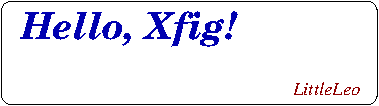
\includegraphics{hello}
  \caption{利用 Xfig 制图}
  \label{fig:xfig1}
\end{figure}

大学之道,在明明德,在亲民,在止于至善。知止而后有定;定而后能静;静而后能安;安
而后能虑;虑而后能得。物有本末,事有终始。知所先后,则近道矣。古之欲明明德于天
下者,先治其国;欲治其国者,先齐其家;欲齐其家者,先修其身;欲修其身者,先正其心;
欲正其心者,先诚其意;欲诚其意者,先致其知;致知在格物。物格而后知至;知至而后
意诚;意诚而后心正;心正而后身 修;身修而后家齐;家齐而后国治;国治而后天下
平。自天子以至于庶人,壹是皆以修身为本。其本乱而未治者 否矣。其所厚者薄,而其所
薄者厚,未之有也!

\hfill \pozhehao《大学》


\subsubsection{多个图形}
\label{sec:multifig}

如果多个图形相互独立,并不共用一个图形计数器,那么用 \verb|minipage| 或者
\verb|parbox| 就可以。否则,请参看图~\ref{fig:big1-subcaptionbox},它包含两个小图,分别是图~\ref{fig:subfig1} 
和图~\ref{fig:subfig2}。推荐使用\verb|\subcaptionbox|,
因为可以像图~\ref{fig:big1-subcaptionbox} 那样对齐子图的标题,
也可以使用\textsf{subcaption}宏包的\verb|\subcaption|(放在minipage中,用法同\verb|\caption|)
或是 subfigure 、 subtable环境,像图~\ref{fig:big1-subfigure},不要再用 \verb|\subfloat|、
\verb|\subfigure| 和 \verb|\subtable|。
\begin{figure}[h]
  \centering%
  \subcaptionbox{第一个小图形\label{fig:subfig1}}
  [3cm] %标题的长度,超过则会换行,如下一个小图。
    {
\includegraphics[height=3cm]{thu-fig-logo}}
      \hspace{4em}%
  \subcaptionbox{第二个小图形,注意这个图略矮些。如果标题很长的话,它会自动换行\label{fig:subfig2}}
      {
\includegraphics[height=2cm]{thu-text-logo}}
  \caption{包含子图形的大图形(subcaptionbox示例)}
  \label{fig:big1-subcaptionbox}
\end{figure}
\begin{figure}[h]
  \centering%
  \begin{subfigure}{3cm}
    
\includegraphics[height=3cm]{thu-fig-logo}
    \caption{第一个小图形}
  \end{subfigure}
  \hspace{4em}%
  \begin{subfigure}{0.5\textwidth}
    
\includegraphics[height=2cm]{thu-text-logo}
    \caption{第二个小图形,注意这个图略矮些。subfigure中同一行的子图在顶端对齐。}
  \end{subfigure}
  \caption{包含子图形的大图形(subfigure示例)}
  \label{fig:big1-subfigure}
\end{figure}
古之学者必有师。师者,所以传道受业解惑也。人非生而知之者,孰能无惑?惑而不从师,
其为惑也,终不解矣。生乎吾前,其闻道也固先乎吾,吾从而师之;生乎吾後,其闻道也亦
先乎吾,吾从而师之。吾师道也,夫庸知其年之先後生於吾乎!是故无贵无贱无长无少,道
之所存,师之所存也。

嗟乎!师道之不传也久矣,欲人之无惑也难矣。古之圣人,其出人也远矣,犹且从师而问焉;
今之众人,其下圣人也亦远矣,而耻学於师。是故圣益圣,愚益愚。圣人之所以为圣,愚
人之所以为愚,其皆出於此乎?爱其子,择师而教之,於其身也,则耻师焉,惑焉。彼童子
之师,授之书而习其句读者,非吾所谓传其道、解其惑者也。句读之不知,惑之不解,或师
焉,或不焉,小学而大遗,吾未见其明也。巫医、乐师、百工之人不耻相师,  士大夫之族
曰“师”曰“弟子”之云者,则群聚而笑之。问之,则曰:彼与彼年相若也,道相似也,位
卑则足羞,官盛则近谀。呜呼!师道之不复,可知矣。巫医、乐师、百工之人。吾子不齿,
今其智乃反不能及,其可怪也欤!圣人无常师。孔子师郯子、苌子、师襄、老聃。郯子之徒,
其贤不及孔子。孔子曰:“三人行,必有我师。”是故弟子不必不如师,师不必贤於弟子。
闻道有先後,术业有专攻,如是而已。

如果要把编号的两个图形并排,那么小页就非常有用了:
\begin{figure}
\begin{minipage}{0.48\textwidth}
  \centering
  
\includegraphics[height=2cm]{thu-whole-logo}
  \caption{并排第一个图}
  \label{fig:parallel1}
\end{minipage}\hfill
\begin{minipage}{0.48\textwidth}
  \centering
  
\includegraphics[height=2cm]{thu-whole-logo}
  \caption{并排第二个图}
  \label{fig:parallel2}
\end{minipage}
\end{figure}

李氏子蟠,年十七,好古文、六艺,经传皆通习之,不拘於时,学於余。余嘉其能行古
道,作师说以贻之。

\hfill \pozhehao 韩愈(唐)


\cite{IEEE-1363}


%%% 其它部分
\backmatter

% 本科生要这几个索引,研究生不要。选择性留下。
\makeatletter
\ifthu@bachelor
  % 插图索引
  \listoffigures
  % 表格索引
  \listoftables
  % 公式索引
  %\listofequations
\fi
\makeatother

% 参考文献
\bibliographystyle{thubib}
\bibliography{ref/refs}


% 致谢
%%% Local Variables:
%%% mode: latex
%%% TeX-master: "../main"
%%% End:

\begin{ack}
  衷心感谢导师 xxx 教授和物理系 xxx 副教授对本人的精心指导。他们的言传身教将使
  我终生受益。

  在美国麻省理工学院化学系进行九个月的合作研究期间,承蒙 xxx 教授热心指导与帮助,不
  胜感激。感谢 xx 实验室主任 xx 教授,以及实验室全体老师和同学们的热情帮助和支
  持!本课题承蒙国家自然科学基金资助,特此致谢。

  感谢 \thuthesis,它的存在让我的论文写作轻松自在了许多,让我的论文格式规整漂亮了
  许多。
\end{ack}


% 附录
\begin{appendix}

\chapter{书面翻译}
\label{chap:translation}
\begin{center}  
  \Large{文档结构相似性算法调研}
\end{center}

\section*{摘要}
  这篇论文对文档结构相似性算法做了简明的调研,包括优化的树编辑距离算法和各种近似
  算法。这些近似算法包括简单加权标签相似度算法,文档结构的傅里叶变换,和将连续序
  列技术应用到结构相似度计算上。我们展示了三个令人惊奇的结果。第一,傅里叶变换的
  方法是所有近似算法中最不精确的一个,同时也是最慢的一个。第二,优化的树编辑距离
  的算法并不一定是最好的用来将不同网站的网页进行聚类的算法。第三,对于许多应用来
  说,最简单的结构的近似可能是最有用也是最有效率的机制。
\section{简介}
随着万维网上大量的文档的出现,自动地处理这些文档,将其应用于信息抽取,近似聚类和
搜索的需求越来越大。在这个领域的主要工作主要集中在文档的内容上。然而,虽然万维网
的继续发展和进化,越来越多的信息被放在结构化的富文本中,从HTML转换到XML。这个结构
化的信息是一个文档意义的重要体现。从文档中辨别出结构上“相似”,或者结构上互
相“包含”的那些文档的方法是一个非常重要那些相关的相似文档关联起来的机制,而这些
文档可能包含不同的文本内容,那些基于文本内容的相似度算法起不到这样的作用。

现在已有几个文档结构在其中起到关键作用的应用。目前的信息提取算法隐式或显式地依赖
文档的结构化元素。结构化的信息能帮助我们将大量的从不同网站上获得的网页整理成一些
可以大致可以比较的集合。这就使得软件能够将可以抽取出正确结果的集合和那些不能抽取
有用信息的集合分离开来。

结构相似度是一个非常重要的话题,有非常多的算法可以计算任意两个文档结构之间的最小
编辑距离。然而,由于这些算法复杂度非常高,通常都需要$O(n^2)$或者更多的时间去计算
距离,因此创造一些更快的,但是距离的计算精确度有些许损失的算法是有可能的。

我们在这篇论文的第二节展示了当前用于检测结构相似度的算法的概述。之后在第三节我们
描述了一个新的基于shingle的计算结构相似度的近似算法。在第四节我们在速度和精确度
上对比了一下这些近似度算法和优化的树编辑距离算法。在第五节中我们用对不同算法特点
的概括进行了总结。

\section{当前研究状况}
基于树的文档结构性相似度的研究已经有很长的历史了。早期基于树的变换检测来
自[1],[2]。近期Shasha [3], [4], [5]和Chawathe [6],[7]做了一些关于树到树变换的
研究,主要集中在如何创建一个最小的脚本用来进行树之间的转换。在将一些基于结构的相
似度计算修改成半结构的格式方
面也有很多的尝试,包括NiagraCQ [8],Xdiff [9],适用
于XML的Xyleme [10],[11],以及AIDE [12],[13]和适用
于HTML的ChangeDetector\textsuperscript{\texttrademark}。

之前关于HTML文档相似度的工作大部分集中在了内容相似度上,页面分段[15]技术也是一样。
目前的结构相似度集中在了XML的Schema的相似度上。DTD相似度研究集中在对成对的文档和
未知但相似的DTD的近似度计算上。这要求每两篇文档比较一次需要$O(n^2)$的计算复杂度。
其他的工作将文档之间结构相似度的问题转化为用傅里叶变换的时间序列的相似度,实现上
采用快速傅里叶变换以实现$O(n\times lgn)$的复杂度。

在这篇论文中,我们引进了一个将shingle技术应用在衡量文档结构相似度上的方法。这要
求用$O(k)$的复杂度去创造一个shingle文档(在这里$k$表示节点的个数),以及提供常数
时间的复杂度进行文档之间的比较。在计算时间上的节省是通过损失计算精确度的得到的,
实际可以任意减小精确度以满足不同的要求。第四节比较了这个技术与其他近似算法在不同
的数据集上的表现。

\subsection{近似算法}
这里我们提供一个对不同类型的用于计算文档相似度算法的概述。我们将描述的衡量标准包
括树编辑距离,标签距离,傅里叶变换和路径相似度。shingle技术的动机和算法我们将在
第三节给出。

树编辑距离相似度。一些作者提供了一些计算两个树之间优化的树编辑距离的算法。这篇论
文使用Nierman和Jagadish [16]描述的动态编程实现。一般来说,编辑距离衡量的是将一个
树转换为另一个树所要求的插入,删除和更新的最少的节点个数。通过将编辑操作的次数和
较大的那个文档的节点个数之间进行归一化,可以将其转换为相似度的衡量标准。令$N_i$为
文档$D_i$的树形表示的节点集合,于是
\[
TED(D_i,D_j)=\frac{editDistance(D_i,D_j)}{max(|N_i|,|N_j|)}
\]

标签相似度。标签相似度可能是结构相似度最简单的度量方法,因为它只衡量两个标签集合
之间的近似程度。在XML文档中,标签是schema的一个组成部分,使用一个类似标签集合的页
面schema也很有可能类似。两个文档的标签集合可以用来测量它们的重合程度。令$T_i$为
文档$D_i$所包含的标签集合,$T_J$为文档$D_j$包含的标签集合。两个页面的简单的标签
相似度为$T_i$和$T_j$的交集和并集的比例。

然而,由于各种原因,这并不令人满意。一个关键的问题是遵循一个相同schema的页面,比
如HTML,只有一个非常有限的不同标签的个数;一个页面可能包含非常多的一个特殊的标签,
但是用于比较的页面只包含相对很少的这个标签。为了补偿标签频率,我们可以引入一个加
权的相似度度量。令$t_{ik}$为$T_i$的一个成员,$w_{ik}$为标签$t_{ik}$在文档$D_i$中
出现的次数。此外,令$t_{jk}$为$T_j$中对应的标签,$v_{jk}$为$t_{jk}$在文档$D_j$中
出现的次数。如果有$n$个互不相同的标签同时出现在文档$D_i$和$D_j$中,加权标签相似
度可以表示为:
\[
WTS(D_i,D_j)=\frac{\sum_{k=1}^n2*min(w_{ik}, v_{jk})}{\sum_{k=1}^n(w_{ik}+v_{jk})}
\]

由于这个仅包含每个文档中的标签集合,结构相似度的精确性与使用的标签无关。因此,这
个度量方法在类似HTML的环境中应该只有非常低的精确度,这些环境标签集合是很有限的,
但是结构却变化非常大。它在一些都遵循一个小的schema集合的文档上有可能变得更加精确,
因为这些schema限制了文档结构的变化。

傅里叶变换相似度衡量。Flesca \textit{et al.} 引入傅里叶变换作为计算文档相似度的
一个手段。基本的想法是将一个文档的开始标签和结束标签以外的全部信息去掉,只保留一
个表示结构的骨干。然后将这个结构转化为一个数字序列。将这个数字序列视为时序序列,
然后使用傅里叶变换将其转化到频域。最终,两个文档之间的距离可以通过两个信号的幅度
差别进行计算。

这个算法有几个对结果有重大影响的关键组成部分。像一开始所说的,文档结构的编码采用
一个独特的(序列的)正数来表示每一个开始标签,用负数来表示对应的结束标签。属性被
当做标签。注意到这个意味着为了比较两个文档,标签的数字映射必须在每个文档中都是一
样的。Flesca \textit{et al.}选择了一个文档$d$的多层的编码,将其映射成一个序列
$[S_0,S_1,\dots,S_n]$,其中
\[
S_i=\gamma(t_i)\times expF(t_i) + \sum_{t_j\in nest_d(t_i)}\gamma(t_j)\times expF(t_j)
\]
其中$\gamma(t_i)$是一个对应于第$i^{th}$个标签的整数,
$expF(t_i)=B^{maxdepth(D)-l_{t_i}}$是一个决定标签权重的指数因子,$B$是一个固定的
底,$maxdepth(D)$是正在比较的文档的最大深度,$l_{t_i}$是第$i^{th}$个标签的深度,
$nest_d(t_i)$是$t_i$的祖先集合。

最终的两个文档$d_1,d_2$的距离度量通过傅里叶变换定义为
\[
dist(d_1,d_2)=(\sum_{k=1}^{M/2}(|[FFT(h_{1})](k)|-|[FFT(h_2)](k)|)^2)^{\frac{1}{2}}
\]
其中$FFT$傅里叶变换关于同时出现在$h_1$和$h_2$中频率的插值,$h_1$是$d_1$对应的信
号,$M$是出现在插值中的点的个数。

这个方法有一些困难的地方。第一,FFT要求点的个数是2的幂。一个DFT实现使用了和文档的
时序表示一样多的点,意味着DFT和FFT近似算法的精度是不一样的。对于我们的比较而言,
我们发现了FFT当成DFT时是$O(n^2)$的,在实践中它比树编辑距离算法更慢,而且DFT的精
度比FFT的精度要低。

第二,调和标签映射的要求和预先计算用于比较文档的最大深度意味着需要有根据单一文档
来预先计算这个算法的任意部分的能力,以减小成对比较所需的时间。

第三,傅里叶变换典型的用法是在重复的无限时间序列上。我们所碰到的那些文档是有限的。
为了可以使用这个变换,我们必须将从文档中提取的时间序列扩展为无限重复的。对于原始
文档这意味着什么以及这个对于比较有那些影响我们都不清楚。

\section{路径shingle}
使用优化的树编辑距离算法的问题在于它在大的文档集上代价非常大。目前所展示的近似算
法要么不够直观(傅里叶变换),要么只提供了一个粗略的相似度度量(加权标签算法)。
我们感到需要有一个可以根据应用来调整精度的快速的近似算法。

Shingle是Broder在[15]中为计算文本文件相似度和包含度而引入的技术。这个技术减小了文
档中词或者标记的集合,将其变成一个散列的列表,能够直接和另一个文档进行比较,通过
集合的差集,并集和交集来计算相似度或者包含度。

更进一步地,shingle集合的子集,叫做sketch,可以用于计算文档的相似度。直观地
说,sketch是一个页面的随机采样的一段文本。关键在于由于随机映射在所有的页面中都是
一样的,而且结果是排好序的,这些样本是可以直接在不同的页面之间进行比较。页面采样
的重合度意味着整个页面的重合程度。

我们将展示如何修改这个技术,将其应用到文档的结构中。这使我们可以在线性时间计算文
档结构相似度。通过稍微减小精度,可以实现常数时间的任意大小的文档之间的比较。

\subsection{路径相似度}
为了创建一个适用shingle技术的结构编码,我们必须找出一个方法去创建一个标记的列表,
用于表示这个结构。一些自然的选择,比如使用深度优先或者广度优先的堆编码,因为用于
表示树的标记列表本身的不分段特性从而证明是不合适的。这意味着当一个分支结束和另一
个分支开始的时候,覆盖序列的窗口不能被辨别出来。覆盖这些的窗口不能精确表示原始文
档的任一部分。为了找到用于这种编码的合适的分段方法,衍生了另一个自然的编码方法:
路径。

半结构化的文档(HTML和XML)可以被看成一个由分支和从根到叶的路径组成的序列。为了我
们的目标,我们将任意的部分路径,即从根到文档中任意的节点组成的路径也认为是一个标
记。一个树可以用一个这些标记的序列来表示。比如,HTML中最简单的树有一个title和
body元素,可以被编码为:\\
/html\\
/html/head\\
/html/head/title/\\
/html/head/title/[text]\\
/html/body
/html/body/[text]

路径相似度衡量两个不同文档之间的路径的相似度。一个路径被定义为一个从根节点开始,
到叶子节点结束的相连的节点列表。路径相似度可以从多种方式进行度量:二元的,路径要
么相等或者不相等;部分的,在每个路径中可以比较的节点的数目是知道的;或者加权的,
节点根据它到根的距离进行加权。

部分路径相似度需要很大的计算代价。因为两个树的路径有$n!$种可能的映射,用穷举的算
法来产生优化的相似度分数是不可行的。二元的相似度代价要小很多,因为在一个版本中的
每一个独特的路径可以通过数据库的join技术来匹配另一个版本中的等价路径。相似度可以
通过匹配上的路径个数和两个树总的路径数的比例来计算。

\subsection{将shingle应用到路径上}
一个shingle是一个从文档中得到的连续的标记的子序列。两个文档的相似性定义为
\[
r(D_i,D_j)=\frac{S(D_i,w)\cap S(D_j,w)}{S(D_i,w)\cup S(D_j,w)}
\]
然而$S(D_i,w)$是从文档$D_i$创建长度为$w$的shingle的操作符。类似地,文
档$D_i$和$D_j$的包含度定义为
\[
c(D_i,D_j)=\frac{S(D_i,w)\cap S(D_j,w)}{S(D_i,w)}
\]

为了方便和快速的处理,shingle可能通过散列函数转换成数字。这个散列函数应该有较高的
可信度使得两个shingle散列成一个数的冲突的可能性变得很小。让散列的空间显著大
于shingle的空间可以使得构造这样一个合适的散列函数变得容易很多。依据一个shingle中
标记的个数(或者窗口的长度),这可能会非常微妙。

一个将结构化比较的复杂度减小到$O(1)$的关键技术是每个文档只保留一个相对小的sketch。
从[15]中我们可以看到从一个shingle集合的排列中进行随机采样得到的样本可以被当成两
个文档之间相似度的无偏估算子。一个有效的实现这个的办法是通过伪随机数生成算法来散
列值,将结果排序,然后选择最小的$k$的结果。

为了将shingle应用到路径结构中,我们定义$S(D_i,w)$如下:对于$D_i$的树形表示中的每
个节点,计算从根到该节点的路径;根据这个(部分)路径的标签名列表创建一个散列;将
该散列加入到当前窗口;窗口向前滑动一个单位(即将窗口的第一个散列值去掉)。。

注意到根据定义,shingle集合可能是一个集合或是一个包——类似于标签相似度和加权标签相
似度之间的差别。于是就出现了使用一个集合来包含shingle会显著减小shingle的表达能力,
并将更大的误差引入到估计中。

我们测量了路径shingle和部分路径shingle的精度。比较是在使用无穷的$k$的不同的窗口大
小下进行的。用来比较是数据是从\texttt{my.yahoo.com}下载的在两年时间内的典型的网页
快照。结果显示小的窗口大小(从1到4)对精度没有影响:两个聚类都没有错误,四个聚类
只引入百分之三的错误。用来比较的shingle个数的不同并不影响聚类的效果。$k$的值从10
测试到了1000,以及一个无穷数量的shingle。所有的都显示了错误在百分之十之内。

\section{实验}
在这一节中我们经验性地评价不同的近似算法与树编辑距离相比的精度,同时还比较了不同
的近似算法的性能。

所有的实验都是在一个配置了速龙双核2G赫兹的处理器,2.4Linux内核的工作站上运行。算
法使用Java实现的,在Sun 1.4.2 JVM上执行。所有的算法都采用了页摘要数据结构来实现,
该数据结果比DOM树表示有很大的性能提升。性能的测量是取10次运行的平均值。

根据聚类进行比较。聚类是在树编辑距离的基础上用来衡量不同度量之间的效果的。树编辑
距离是可证明的一个两个树之间的最佳的编辑距离。我们假定这是最好的相似度度量。其他
的算法会产生一些不同的距离度量,不能直接和一个编辑距离进行比较。然而,如果一个大
的文档集合是根据某个度量方法来聚类的,这些通过不同的度量方法产生的聚类是可以通过
给定同一个聚类方法进行比较的。换句话说,如果两个文档通过树编辑距离判断是相似的,
那么其他的度量也应该认为这两个文档是相似的,或者恰恰相反。

我们可以将一个在一个近似算法中被放在一个shingle聚类中,而在树编辑距离算法中放到
另一个类中的归类成错误文档。这个错误度量有一些缺点。比如,一个文档集合被分成两个
聚类,任何度量都会有严格小于50\%的最大错误率。一般地,随着聚类数目$n$的增长,最
大错误率严格小于$1-\frac{1}{n}$。

我们用两个数据集进行聚类。第一个是从500个XML文档中综合生成的集合。这个集合建模一
个书仓库,每个文档都列出一个书对应的作者,发行商和发行时期。文档之间唯一的结构差
别在于这本书的作者的个数。

每个度量方法都用来度量两个文本之间距离。文档根据这些距离通过开$k-means$进行聚类。
通过每种度量得到的聚类与树编辑距离得到的聚类进行比较,计算一个错误估计。结果显示
在Table I中。
{\centering
  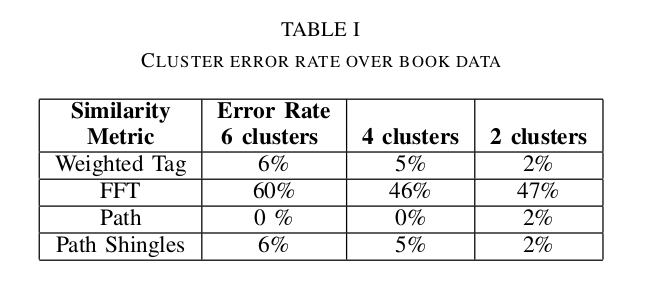
\includegraphics[width=\textwidth]{translationTable1}
}
我们测试了最多6个聚类,因为这个数据集中根据书籍的作者数量,有6个自然的聚类。我们
期望加权标签度量有较低的错误率,因为这些数据之间的结构差异只有\texttt{author}这
个标签出现的次数。

第二个数据集是一系列从以下网站得到的快
照:cnn.com,corona.bc.ca,news.gnome.org,10-10phonerates.com和my.yahoo.com。快
照是2001到2003两年期间的,大概是每天一次。冗余的快照(由MD5签名决定)被移除了,每
个站点的快照集合取样20份页面。一样的聚类算法用在这些文档上,只有这次我们有一个预
定义好的聚类(通过网站),并且可以将每个算法同这些预定义好的聚类进行比较。结果显
示在Table II中。{\centering
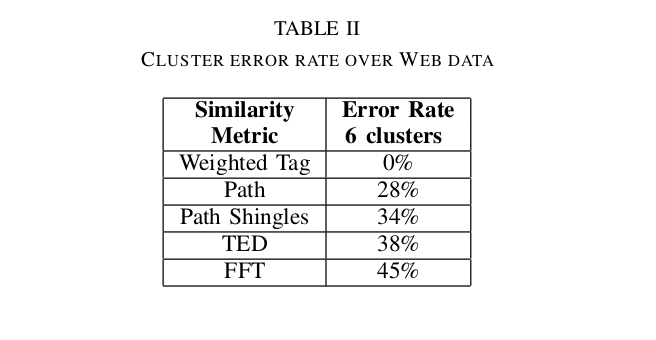
\includegraphics[width=\textwidth]{translationTable2}
}

这个错误率好像异常地高,特别是对于我们在其他测试中用来当做基准的树编辑距离算法。
我们推测这个错误率是由于HTML的结构中用来呈现给用户内容的词汇相对较小。路径和路
径shingle度量比树编辑距离性能要好,但也比预期的要差。这可能是因为它们使用了部分路
径来描述树的结构。很深的树在顶部区域可能会呈现很多相似的结构,导致两个来自不同站
点的树的相似度可能会互相偏向。FFT度量方法的糟糕的性能不能给出一个简单的解释。可以
说依据相同的最开始的一批标签(\texttt{html},\texttt{head}和\texttt{body}),每个
网页都是极度相似的信号,在叶子层面也是相似的构造(标签列表和文本)。然而,这个转
换使得我们难以找出是网页的哪一些特征导致它们变得如此相似。

作为最后的比较,我们检查了以上表格中从一个站点来的快照。这会在比如监测一个页面随
着时间变化的时候很有用。我们选择my.yahoo.com,因为里面的内容会定期发生变化,但是
结构上随着时间的变化很缓慢(比如,当一个新的图片被加入到一些特点的假日)。我们再
次把使用近似算法和树编辑距离产生的聚类进行比较。{\centering
  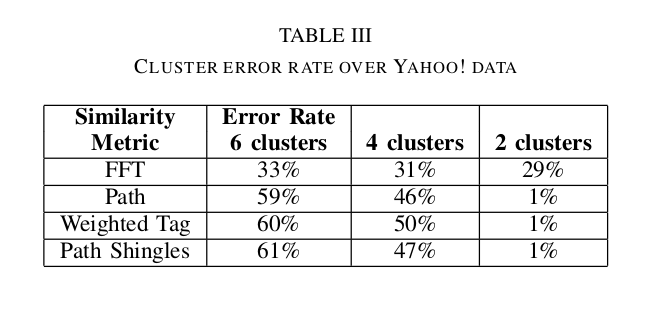
\includegraphics[width=\textwidth]{translationTable3}
}

我们观察到除了FFT以外的大部分近似算法在小的聚类大小上都有非常低的错误率,但是错误
率在聚类的规模变大时会激增。观察一下描述树编辑距离聚类和FFT聚类以及路径/路径
shingle聚类之间映射变化的矩阵是有意义的。Table IV描述了FFT聚类和树编辑距离聚类的
不同,Table V描述了路径聚类和树编辑距离聚类之间的不同。
{\centering
  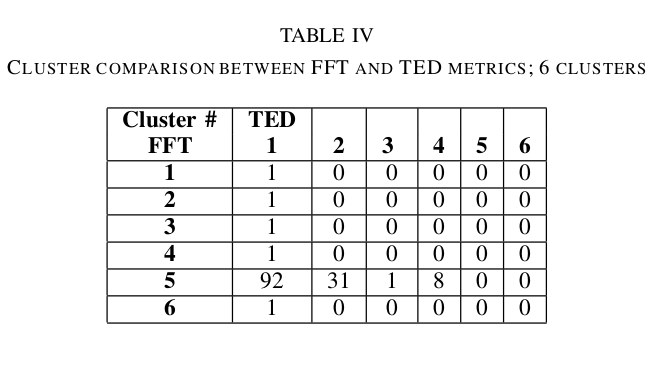
\includegraphics[width=\textwidth]{translationTable4}
}

从这两个矩阵我们可以推导出FFT度量会倾向于将所有的数据点聚成一个类别,因此不提供一
个有效的分辨相似网页的能力。在另一方面,路径度量(路径shingle和加权标签度量实际是
一样的)比树编辑距离更有分辨能力,能够比树编辑距离分出更好的类别。尽管这些实验中
将这种情况标为了错误,它可能有很重要的分辨那些感觉上不一样,但在相同的编辑距离内
的树的功能。

最惊奇的观察在于加权标签的相似度度量方法,一开始我们认为是一文不值的东西,却能和
复杂很多的技术达到一样的精确程度。这可能可以归因为大部分实验是在来自一个站点的相
对同构的页面上进行的(就像书籍数据集或者Yahoo!数据集的情况一样),或者可以归因为
非同构的站点为了突出它们的对比而使用了不同HTML标签子集。另一个观察是傅里叶变换技
术在很简单的数据集上表现也很差。这就使得我们认为尽管这是一个将结构转换为一个更简
单的用于比较的格式的想法,但是它并不适用与文档结构,无论是从分析上还是实验上。

\subsection{性能比较}
选择一个近似算法的主要原因是为了将速度提高到一个可以接受的水平,因为最优的算法太
慢了。文档聚类用于数据抽取或者搜索和获取方法,提供了一个结构化相似度的很好的例
子。用于精度估计的相对小的数据集说明了近似算法在计算近似相似度上的有效性。Figure
1展示了不同算法在书籍文档的数量对数增长时的相对代价。

聚类的时间是在一个小于一千比特的较小的文档上计算的。为了更好地理解计算两个文档之
间差异的代价,我们比较了在TCP-H基准测试数据上的每个度量方法的代价。这个数据是
由Toxgene [19]XML文档生成器随机生成的。我们修改了生成器的参数以便产生包含原始数据
集合1\%,5\%,10\%,15\%,20\%,和25\%的文档。这个生成器跑两次,在每个分数上产生
两个不同的文档。结果在Figure 2中。

我们可以看到树编辑距离算法比任何其他的近似算法都要慢好几个数量级。FFT算法也显示
出了尽管它用很大的精度换来了速度,它仍然比加权标签或者路径shingle方法慢一个数量
级,后两者的精度还显著更高。

大文件支持。以空间换时间的优化对于小到中型大小的文件都工作地很好,但是树编辑距离
在其数据结构会超过物理内存的大文件上明显变慢。当物理内存被耗尽,机器被迫开始使用
交换内存——这个会慢好几个数量级。

shingle在创建常数大小的大文件指纹时有优势,消除了在计算时在内存中维护复杂数据结构
的需要。

shingle还可以部分调优,就算是因此取了原始的指纹。给定一个窗口散列的集合,只有最前
面的$k$个需要比较。用于比较的散列的数目可以调整,把精度用来换速度和空间。这就使得
对于更低精度的比较,一次性可以有更多的指纹在内存中驻留。

\section{总结}
我们展示了一些测量文档结构相似度的算法,比较了它们的精度和性能。我们有了一些有趣
的发现。

第一,我们提供了一个对[17]中所描述的傅里叶变换的实验性的批判。尽管相比最优化树编
辑距离算法,傅里叶变换方法是一个更快的方法,但这个方法没有提供在不同情境中的一个
精确的相似度衡量。此外,这个技术的性能也通常比其他更直观的相似度计算方法要差。

第二,对于很多结构相似度的应用来说,最简单的计算标签数量的方法提供了最好的性能情
况下的一个可以接受的精度。我们一开始将加权标签相似度当成一个不重要的计算结构相似
度最快的近似方法。然而,结果是它可以和其他任何近似算法表现一样好,甚至更好。尽管
它没有像树编辑距离方法一样(匹配的相同子树),或者路径shingle方法一样(子结构包含
性)提供一定的结构特征,但是对于不需要这些特征的应用来说,这个算法既快又有辨别
力。

最后,我们基于文档结构中的路径展示了一个新的相似度度量。我们通过应用shingle技术,
可以从任意的文档中创建常数大小的表示方法,使得比起其他相似度度量,聚类方法可以应
用到大很多的文档集合中。此外,这种度量具有在一个大文档集合中搜索子结构和在基于树
的文档集合中做一些结构化的挖掘的能力。

\section*{致谢}
作者要感谢Chunk Baldwin和Ghaleb Abdulla,他们刺激了这些话题之间的对话。作者还要感
觉Daniel Rocco,他搭建了第一个实验框架,并帮助开发了页面摘要数据结构,作为许多算
法的基础。

这个工作是基于No. W-7405- ENG-48. UCRL-CONF-202728法令,在美国能源部的保护下,
在University of California Lawrence Livermore National Laboratory进行的,

\section*{参考文献}
\begin{enumerate}[{[}1{]}]
\item K. C. Tai, “The tree-to-tree correction problem,” Journal of the ACM,
  vol. 26, no. 3, 1979.
\item S. Y. Lu, “A tree-to-tree distance and its application to cluster
  analysis,” IEEE Trans. Pattern Anal. Mach. Intell. PAMI-1, no. 2, 1979.
\item D. Shasha and K. Zhang, “Fast algorithms for the unit cost editing
  distance between trees,” Journal of Algorithms, no. 11, 1990.
\item K. Zhang, D. Shasha, and J. T.-L. Wang, “Approximate tree matching in the
  presence of variable length don’t cares,” J. Algorithms, vol. 16, no. 1, pp.
  33–66, 1994. [Online]. Available: citeseer.nj.nec.com/zhang93approximate.html
\item D. Shasha and K. Zhang, “Approximate tree pattern matching,” in Pattern
  Matching Algorithms. Oxford University Press, 1997, pp. 341–371. [Online].
  Available: citeseer.nj.nec.com/95609.html
\item S. Chawathe, A. Rajaraman, H. Garcia-Molina, and J. Widom, “Change
  detection in hierarchically structured information,” in Proceedings of ACM
  SIGMOD, 1996.
\item S. S. Chawathe and H. Garcia-Molina, “Meaningful change detection in
  structured data,” in Proceedings of the 1997 ACM SIGMOD, 1997, pp. 26–37.
  [Online]. Available: citeseer.nj.nec.com/article/chawathe97meaningful.html
\item J. Chen, D. DeWitt, F. Tian, and Y. Wang, “NiagaraCQ: A scalable
  continuous query system for Internet databases,” in Proceedings of the 2000
  ACM SIGMOD, 2000.
\item Y. Wang, D. DeWitt, and J.-Y. Cai, “X-Diff: An effective change detection
  algorithm for XML documents,” International Conference on Data Engineering,
  2003.
\item A. Marian, S. Abiteboul, G. Cobena, and L. Mignet, “Change- centric
  management of versions in an XML warehouse,” in The VLDB Journal, 2001, pp.
  581–590. [Online]. Available: citeseer.nj.nec.com/marian00changecentric.html
\item G. Cobena, S. Abiteboul, and A. Marian, “Detecting changes in XML
  documents,” in International Conference on Data Engineering, 2002, pp. 41
  –52.
\item F. Douglis, T. Ball, Y.-F. Chen, and E. Koutsofios, “The AT\&T Internet
  difference engine: Tracking and viewing changes on the Web,” in World Wide
  Web, vol. 1, January 1998, pp. 27–44.
\item Y.-F. Chen, F. Douglis, H. Huan, and K.-P. Vo, “TopBlend: An efficient
  implementation of HtmlDiff in Java,” in Proceedings of the WebNet2000
  Conference, San Antonio, TX, November 2000.
\item V. Boyapati, K. Chevrier, A. Finkel, N. Glance, T. Pierce, R. Stokton, and
  C. Whitmer, “ChangeDetector(TM): A site-level monitoring tool for the WWW,”
  in WWW2002, May 2002.
\item A. Z. Broder, “On the Resemblance and Containment of Documents,” in
  Proceedings of Compression and Complexity of SEQUENCES 1997, 1997.
\item A. Nierman and H. Jagadish, “Evaluating structural similarity in XML
  documents,” Fifth International Workshop on the Web and Databases, 2002.
\item S. Flesca, G. Manco, E. Masciari, L. Pontieri, and A. Pugliese, “Detect-
  ing structural similarities between XML documents,” Fifth International
  Workshop on the Web and Databases, 2002.
\item D. Rocco, D. Buttler, and L. Liu, “Page Digest for large-scale Web ser-
  vices,” in Proceedings of the IEEE Conference on Electronic Commerce, June
  2003.
\item D. Barbosa, A. O. Mendelzon, J. Keenleyside, and K. A. Lyons, “Toxgene:
  An extensible template-based data generator for XML,” in SIGMOD Conference,
  2002. [Online]. Available: citeseer.nj.nec.com/525958.html
\end{enumerate}
%%% Local Variables: 
%%% mode: latex
%%% TeX-master: "../main"
%%% End: 

\end{appendix}

% 个人简历
\begin{resume}

  \resumeitem{个人简历}

  xxxx 年 xx 月 xx 日出生于 xx 省 xx 县。
  
  xxxx 年 9 月考入 xx 大学 xx 系 xx 专业,xxxx 年 7 月本科毕业并获得 xx 学士学位。
  
  xxxx 年 9 月免试进入 xx 大学 xx 系攻读 xx 学位至今。

  \resumeitem{发表的学术论文} % 发表的和录用的合在一起

  \begin{enumerate}[{[}1{]}]
  \item Yang Y, Ren T L, Zhang L T, et al. Miniature microphone with silicon-
    based ferroelectric thin films. Integrated Ferroelectrics, 2003,
    52:229-235. (SCI 收录, 检索号:758FZ.)
  \item 杨轶, 张宁欣, 任天令, 等. 硅基铁电微声学器件中薄膜残余应力的研究. 中国机
    械工程, 2005, 16(14):1289-1291. (EI 收录, 检索号:0534931 2907.)
  \item 杨轶, 张宁欣, 任天令, 等. 集成铁电器件中的关键工艺研究. 仪器仪表学报,
    2003, 24(S4):192-193. (EI 源刊.)
  \item Yang Y, Ren T L, Zhu Y P, et al. PMUTs for handwriting recognition. In
    press. (已被 Integrated Ferroelectrics 录用. SCI 源刊.)
  \item Wu X M, Yang Y, Cai J, et al. Measurements of ferroelectric MEMS
    microphones. Integrated Ferroelectrics, 2005, 69:417-429. (SCI 收录, 检索号
    :896KM.)
  \item 贾泽, 杨轶, 陈兢, 等. 用于压电和电容微麦克风的体硅腐蚀相关研究. 压电与声
    光, 2006, 28(1):117-119. (EI 收录, 检索号:06129773469.)
  \item 伍晓明, 杨轶, 张宁欣, 等. 基于MEMS技术的集成铁电硅微麦克风. 中国集成电路, 
    2003, 53:59-61.
  \end{enumerate}

  \resumeitem{研究成果} % 有就写,没有就删除
  \begin{enumerate}[{[}1{]}]
  \item 任天令, 杨轶, 朱一平, 等. 硅基铁电微声学传感器畴极化区域控制和电极连接的
    方法: 中国, CN1602118A. (中国专利公开号.)
  \item Ren T L, Yang Y, Zhu Y P, et al. Piezoelectric micro acoustic sensor
    based on ferroelectric materials: USA, No.11/215, 102. (美国发明专利申请号.)
  \end{enumerate}
\end{resume}

\end{document}
